\documentclass{beamer}

\mode<presentation> {
	\usetheme{Madrid}
	\usecolortheme{default}
	\usepackage{textpos}
	\usefonttheme{default}
	\setbeamertemplate{caption}[numbered]
	\setbeamertemplate{itemize items}[circle]	%square, circle, etc, ...
	\setbeamertemplate{headline}{}				%removes top bar
	\setbeamertemplate{navigation symbols}{}	%remove navigation symbols
	%\setbeamerfont{frametitle}{size=\small}
}

\usepackage[english]{babel}
\usepackage[utf8x]{inputenc}
\usepackage{tikz}
\usepackage{graphicx}
\usepackage{caption}
\usepackage{pgfplots}
%\usepackage{array}
%\usepackage[framed,numbered,autolinebreaks,useliterate]{mcode}
%\usepackage{ragged2e}
%\usetikzlibrary{shapes.geometric, arrows, positioning}
%\tikzstyle{phase} = [rounded corners, text centered, draw=none, fill=none]
%\tikzstyle{arrow} = [thick, ->, >=stealth]


\title[Hedge Cue Detection]{Hedge Cue Detection in Natural Language Text}
\titlegraphic{
\includegraphics[height=2cm,width=2cm]{headers/logo-unifi}}
%\author[M. Lapucci, A. Sortino]{Matteo Lapucci, Alessio Sortino}
\institute[]{{\large Machine Learning}\\\vspace{0.3cm}\textit{University of Florence, Department of Information Engineering}}
\author[A. Sortino, V. Sharma]
{\parbox[c]{1.5in}{Alessio Sortino\\\texttt{\tiny alessio.sortino@stud.unifi.it}} \and 
	\parbox[c]{1.5in}{Vishal Sharma\\\texttt{\tiny vishal.sharma@stud.unifi.it}}}
\date{\today}
\hypersetup{pdfauthor={Alessio Sortino and Vishal Sharma}}

%\AtBeginSection[] {
%	\begin{frame}{Contents}
%		\tableofcontents[currentsection]
%	\end{frame}
%}

\begin{document}
	
	
\frame[plain]{\titlepage} % Print the title page as the first slide

\usebackgroundtemplate
{
	%\includegraphics[width=\paperwidth,height=\paperheight]{background4}
}


%----------------------------------------------------------------------------------------
%	PRESENTATION SLIDES
%----------------------------------------------------------------------------------------
\begin{frame}{Overview}
	\tableofcontents
\end{frame}

\section{Introduction}
\begin{frame}{Introduction}
	\begin{itemize}\setlength\itemsep{1em}
		\item Hedge cue detection is a Natural Language Processing (NLP) 	task that consists of determining whether sentences contain hedges.
		\item These linguistic devices indicate that authors do not or cannot back up their opinions or statements with facts.
		\item This binary classification problem, i.e. distinguishing factual versus uncertain sentences, only recently received attention in the NLP community.
	\end{itemize}
\end{frame}
\begin{frame}{Introduction}
	This project aims to address two task:\\
	\begin{enumerate}\setlength\itemsep{1em}
		\item Learning to detect sentences containing uncertainty
		\item Learning to resolve the in-sentence scope of hedge cues
	\end{enumerate}
	\vspace{0.5cm}
	The model use embedding word vectors, generated by GloVe, to better describe the semantic meaning of words, and LSTM to capture the sequential nature of a sentence.\\
	\vspace{0.5cm}
	The performances achieved by our method are a bit far from today's state-of-the-art, obtaining 60\% of $F$-score on the best binary classifier model, and 32\% on the best model for in-sentence cue detection.
	%\textcolor{red}{TODO: Giustificare l'utilizzo di Glove (sono features che permettono di avere informazioni aggiuntive anche riguardo la "vicinanza" tra parole) e LSTM (permettono di trattare sequenze -- di lunghezza variabile).\\TODO: Aggiungere un \textquotedblleft riassunto" di due righe riguardo ciò che è stato fatto e le performance ottenute. Eventualmente aggiungere un breve confronto con lo stato dell'arte.
	%}
\end{frame}
\begin{frame}{Related Work}
	Different techniques achieve state-of-the-art result on both of our tasks, in particular for the dataset we used:
	\begin{itemize}\setlength\itemsep{1em}
		\item In 2010, Georgescul et al. achieved 60.2\% of $F$-score using a 	Support Vector Machine classifier and employing $n$-grams from annotated cue phrases as features. This method achieved the top performance in the CoNLL 2010 Wikipedia hedge-detection task.
		\item In 2012, Frasconi et al. achieved 61.48\% of $F$-score on classification using a kLog, a kernel-based logical and relational learning.
		\item In 2014, Li et al. achieved 62.9\% of $F$-score on classification using a Hidden Markov Model (HMM).
		\item In 2010, Morante et al. (CoNLL 2010 Wikipedia) achieved 57.3\% of $F$-score on in-sentence cue detection using a memory-based system that relies on information from syntactic dependencies.
	\end{itemize}

\end{frame}

\section{GloVe}
\begin{frame}{Word Representation}
	\begin{itemize}\setlength\itemsep{1em}
		\item Vector Space Models (VSMs) represent words in a continuous space where semantically similar words are mapped to nearby	points.
		\item For example, \textquotedblleft monitor" is embedded ideally nearby \textquotedblleft screen".
		\item VSMs have a long history in Natural Language Processing, but all methods depend in some way how words share semantic meaning if appears in the same contexts. The different approaches that leverage this principle can be divided into two categories:
		\begin{enumerate}
			\item \textit{Count-Based Methods}, e.g. LSA and HAL.
			\item \textit{Prediction-Based Methods}, e.g. word2vec (CBOW and Skip-Gram models) and ivLBL.
		\end{enumerate}
	\end{itemize}
\end{frame}
\begin{frame}{Count-Based Methods}
	The Count-Based Methods for creating word embeddings use low-rank approximations to decompose large matrices made of statistical information about all the corpus.
	\begin{itemize}\setlength\itemsep{1em}
		\item In LSA (Latent Semantic Analysis), rows correspond to words and the columns correspond to different documents. The entries correspond to the number of times a given word occurs in a document.
		\item In HAL (Hyperspace Analogue to Language), rows and columns both correspond to words and the	entries correspond to the number of times a given word occurs in the context of another given word (a \textit{co-occurrence matrix}).
	\end{itemize}
	\textbf{Problem}: frequent words contribute a disproportionate amount to the similarity measure and so some kind of normalization is needed.
\end{frame}
\begin{frame}{Prediction-Based Methods}
	Prediction-Based Methods learn word representations from local context windows instead than all the corpus. The typical model used is \textit{word2vec} of Mikolov et al. (2013). 
	\begin{itemize}
		\item It's a full neural network with a simple single-layer architecture based 	on the inner product between two word vectors.
		\item The target of this model is to maximize the log probability of the next word $w_i$ given the context words $w_k$ in term of a softmax function as a windows scan over the corpus.
	\end{itemize}
	The model is divided in two sub-models:
	\begin{enumerate}
		\item Continuous Bag of Words (CBOW): the target is to predict a word given its context. Good for \textit{small} datasets.
		\item Continuous Skip-Gram: the target is to predict a word's context given the word itself. Good for \textit{large} datasets.
	\end{enumerate}
	\textbf{Problem}: they operate on all the corpus locally.
\end{frame}
\begin{frame}{Global Vectors for Word Representation (GloVe)}
	\begin{itemize}\setlength\itemsep{1em}
		\item The main idea of GloVe is to use the benefits of both methods by counting data while simultaneously capturing the meaningful linear substructures prevalent in prediction-based methods.
		\item GloVe is a global log-bilinear regression model for the unsupervised learning of word representations.
		\item It's been developed by Pennigton et al. (2015) and outperforms other models on word analogy, word similarity, and named entity recognition tasks.
	\end{itemize}
\end{frame}
\begin{frame}{The GloVe Model}
	\begin{itemize}
		\item First of all, word co-occurrence statistics are collected in a word-word co-occurrence matrix $X$. Each element $X_{ij}$ of such matrix represents how many times word $w_i$ appears in context of word $w_j$.
		\item The probability that the word $w_j$ appears near word $w_i$ is:
		$$P_{ij} = P(w_j | w_i) = \frac{X_{ij}}{\sum_{k}X_{ik}}$$
		However, the relationship between two words can be examined by studying the ratio of the probabilities compared to another word, e.g.
		$$\frac{P(solid|ice)}{P(solid|steam)} > \frac{P(gas|ice)}{P(gas|steam)}$$
		\item The model can be written as:
		$$F(w_i, w_j, \widetilde{w}_k) = \frac{P_{ik}}{P_{jk}} \Longrightarrow w_i^T \widetilde{w}_k + b_k + \widetilde{b}_k = \log \left(X_{ik}\right),$$
		where the right member is the solution of the left equation.
	\end{itemize}
\end{frame}
\begin{frame}{The GloVe Model}
	\begin{itemize}
		\item The main drawback of this model is that it weighs all co-occurrences equally, even those that happen rarely or never.
		\item GloVe uses a new weighted least squares regression model:
		$$J = \sum_{i=1}^{V}\sum_{j=1}^{V}f(X_{ij})\left(w_i^T \widetilde{w}_j + b_i + \widetilde{b}_j - \log X_{ij}\right)^2$$
		where $V$ is the size of the vocabulary and $f$ is the weighting function defined as:
		
		\begin{minipage}{0.45\textwidth}
			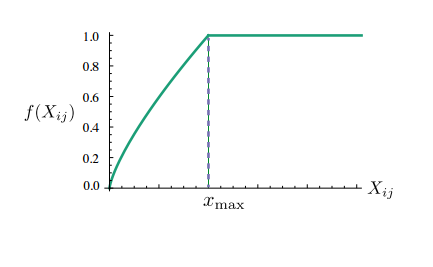
\includegraphics[scale=0.4]{images/glove-fig-1}
		\end{minipage}
		\begin{minipage}{0.3\textwidth}
			\begin{equation*}
			f(X_{ij}) =
			\begin{cases}
			\left(\frac{X_{ij}}{x_{max}}\right)^\alpha & \text{if } X_{ij} < x_{max}\\
			1 & \text{otherwise}
			\end{cases}
			\end{equation*}
		\end{minipage}
	\end{itemize}
 \end{frame}

\section{LSTM}
\begin{frame}{Recurrent Neural Networks (RNNs)}
	\begin{itemize}
		\item When we read a text, we understand each word based on our understanding of previous words. We don't throw everything away and start thinking from scratch again. Our thoughts have persistence.
		\item Recurrent neural networks are networks with loops in them, allowing information to persist.
		\item A recurrent neural network can be thought of as multiple copies of the same network, each passing a message to a successor. 
		\item This chain-like nature reveals that recurrent neural networks are intimately related to sequences and lists.
	\end{itemize}
	\begin{figure}[htbp]
		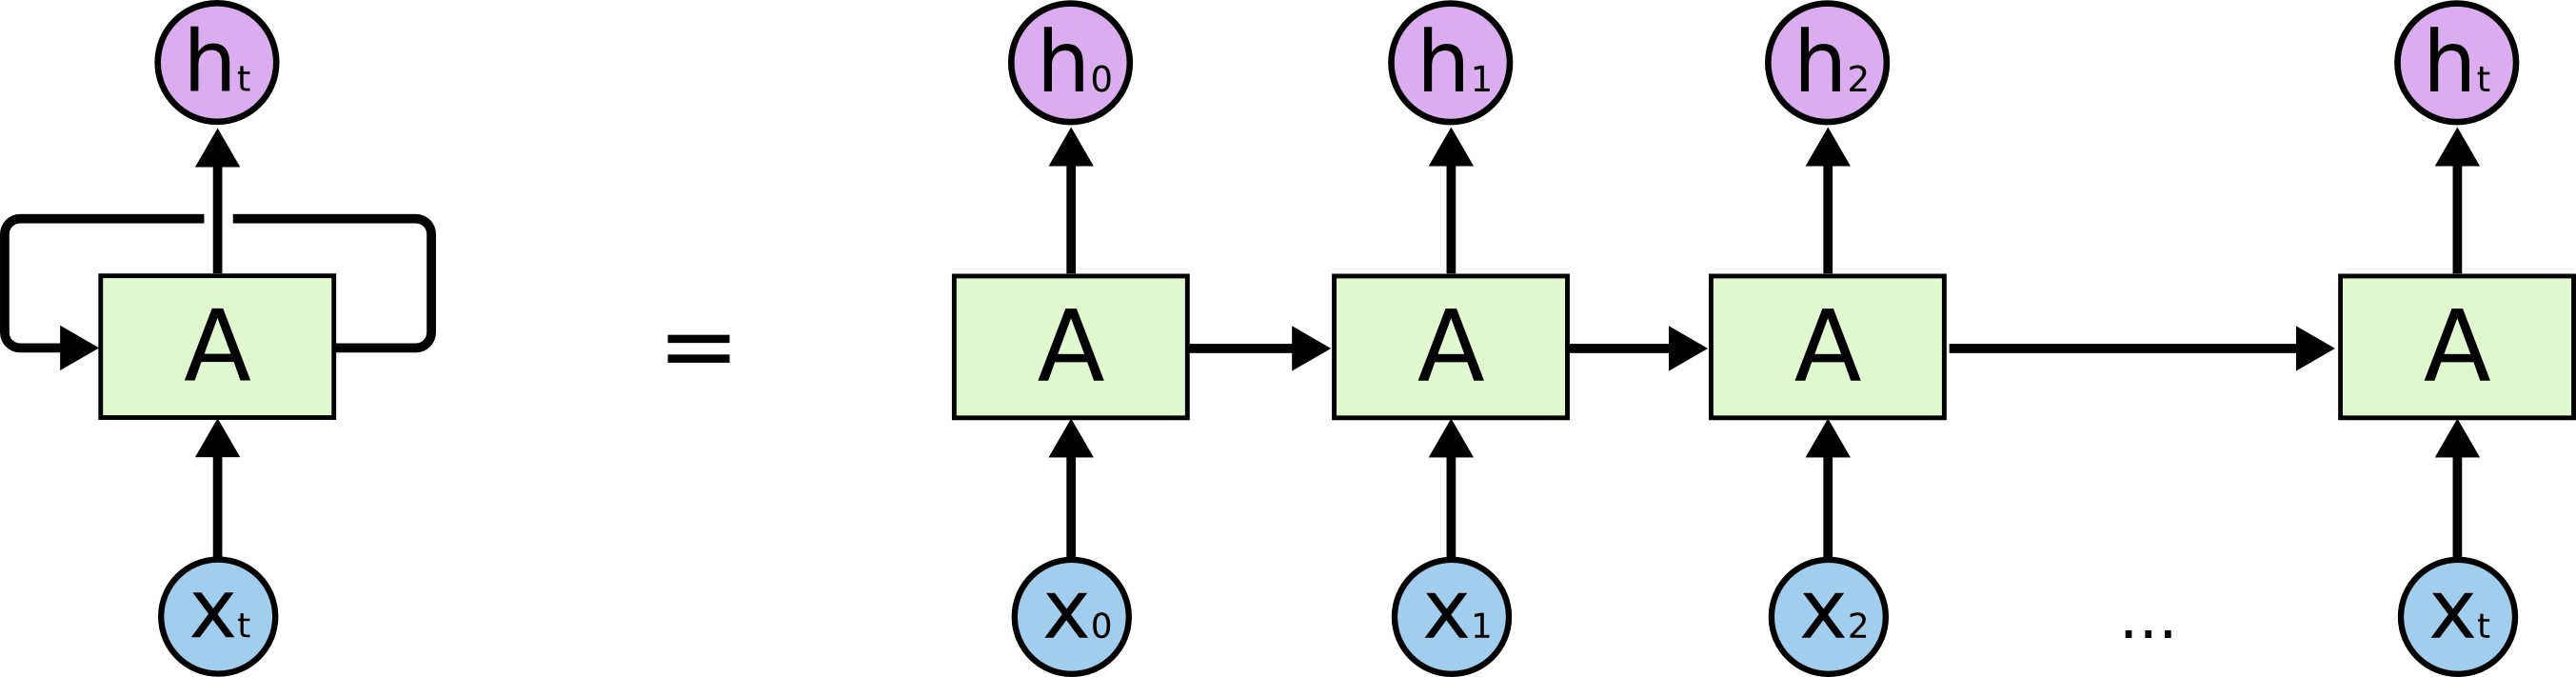
\includegraphics[scale=0.30]{images/RNN-unrolled}
	\end{figure}
\end{frame}
\begin{frame}{Long Short-Term Memory (LSTM) Networks}
	\begin{itemize}
		\item LSTMs are a special kind of RNN, capable of learning long-term dependencies.
		\item LSTMs are explicitly designed to avoid the long-term dependency problem. Remembering information for long periods of time is practically their default behavior, not something they struggle to learn.
		\item LSTMs networks have the form of a chain of repeating modules of neural network.
	\end{itemize}
	\begin{figure}[htbp]
		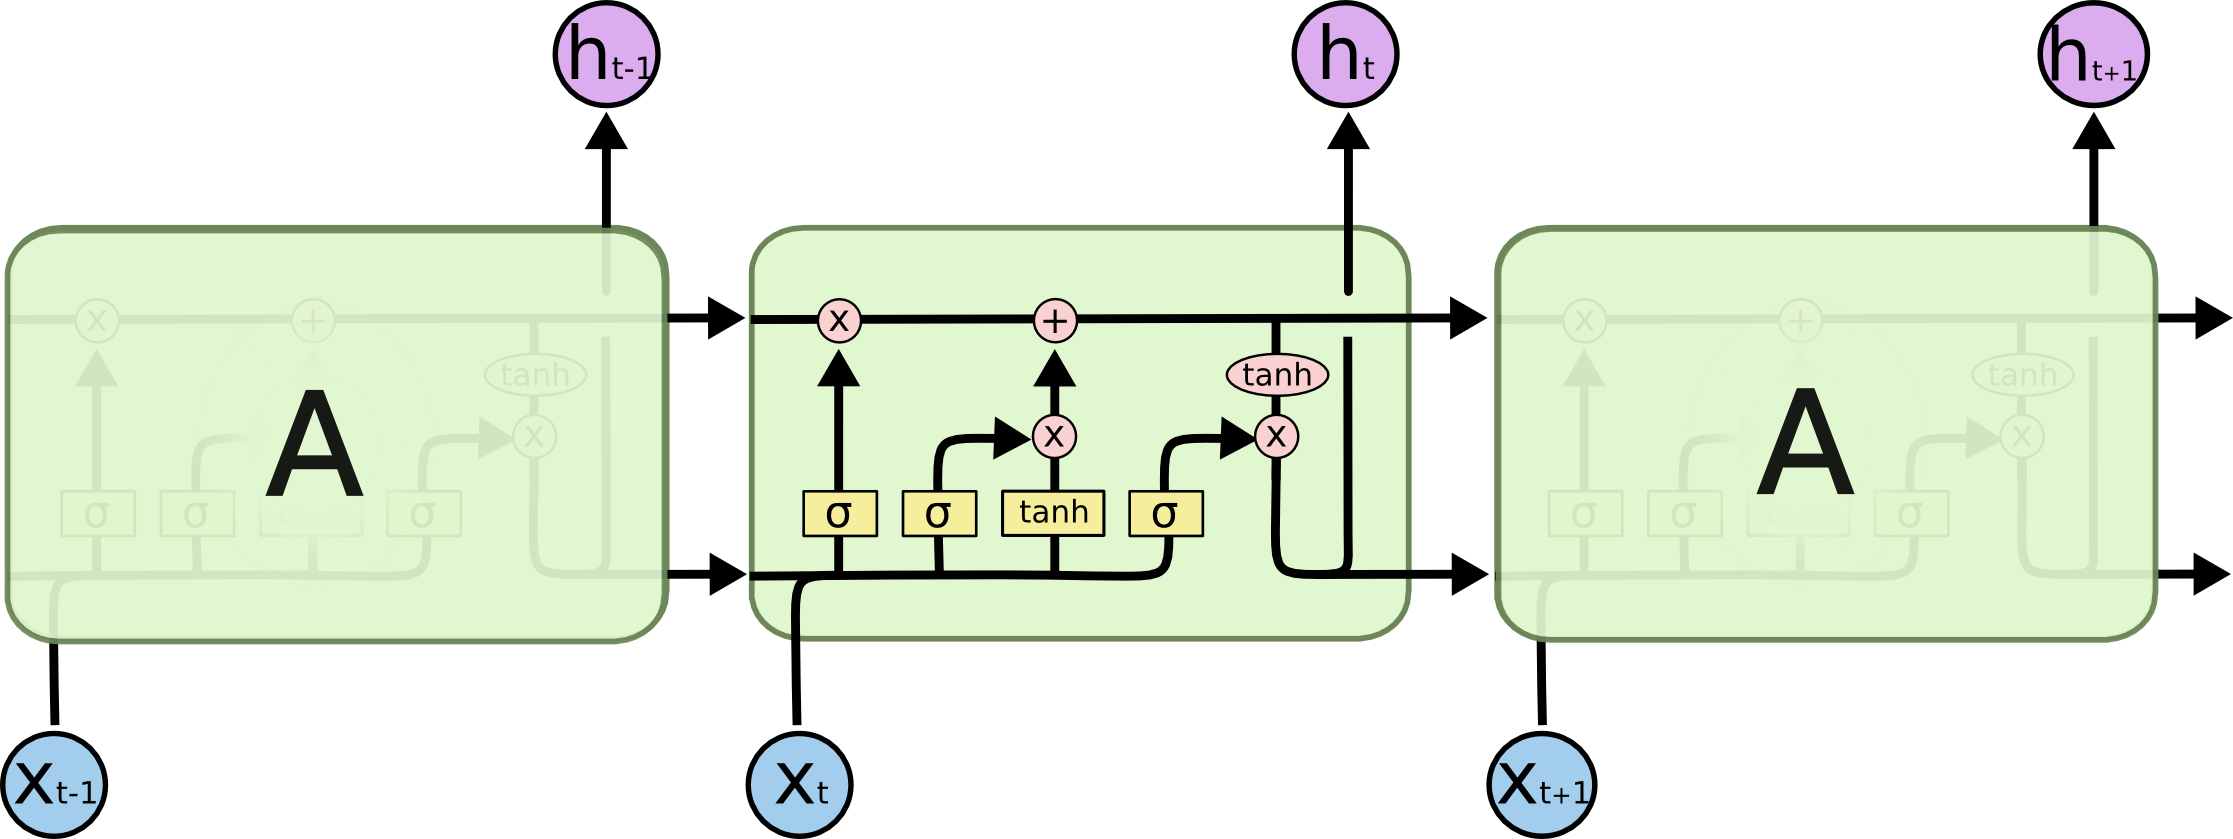
\includegraphics[scale=0.3]{images/LSTM3-chain}
		\caption*{The repeating module in an LSTM contains four interacting layers.}
	\end{figure}
\end{frame}
\begin{frame}{Long Short-Term Memory (LSTM) Networks}
	\begin{itemize}
		\item The key to LSTMs is the cell state, the horizontal line running through the top of the diagram. 
		\item The LSTM does have the ability to remove or add information to the cell state, carefully regulated by structures called gates.
		\item Gates are a way to optionally let information through.
	\end{itemize}
	\begin{figure}[htbp]
		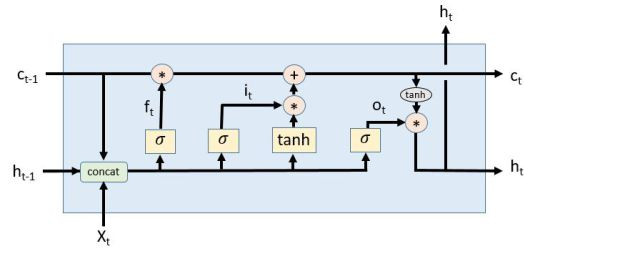
\includegraphics[scale=0.35]{images/lstm_cell.jpg}
		\caption*{LSTM cell.}
	\end{figure}
\end{frame}
\begin{frame}{Long Short-Term Memory (LSTM) Networks}
	There are three types of gates within a unit:
	\begin{itemize}
		\item The \textit{Input Gate} $i_t$ that conditionally decides which values from the input to update the memory state.
		\item The \textit{Forget Gate} $f_t$ that conditionally decides what information to throw away from the block.
		\item The \textit{Output Gate} $o_t$ that conditionally decides what to output based on input and the memory of the block.
	\end{itemize}
	All three of the gates depend on the previous output $h_{t-1}$ on the current input $x_t$.
	%\textcolor{red}{TODO: Add gates equations}
\end{frame}
\begin{frame}{Long Short-Term Memory (LSTM) Networks}
	These are the functions of the LSTM cell, where $\sigma(\cdot)$ is the sigmoid function.
	\begin{eqnarray*}
		i(t) &=& \sigma(W_i \cdot [h_{t-1}, x_t] + b_i)\\
		f(t) &=& \sigma(W_f \cdot [h_{t-1}, x_t] + b_f)\\
		c_t &=& f_t \ast c_{t-1} + i_t \ast \tanh(W_c \cdot [h_{t-1}, x_t] + b_c)\\
		o(t) &=& \sigma(W_o \cdot [h_{t-1}, x_t] + b_o)\\
		h_t &=& o_t \ast \tanh(c_t)
	\end{eqnarray*}
\end{frame}
\begin{frame}{Bidirectional LSTM}
	\begin{itemize}
		\item BLSTM neural network is similar to LSTM network in structure because both of them are constructed with LSTM units. 
		\item The principle of BLSTM is to split the neurons of a regular LSTM into two directions, one for positive time direction (forward states), and another for negative time direction (backward states).
		\item By this structure, the output layer can get information from past and future states.
		\item The final output can be obtained through some operation: sum, concatenation, average, etc.
	\end{itemize}
	\begin{figure}[htbp]
		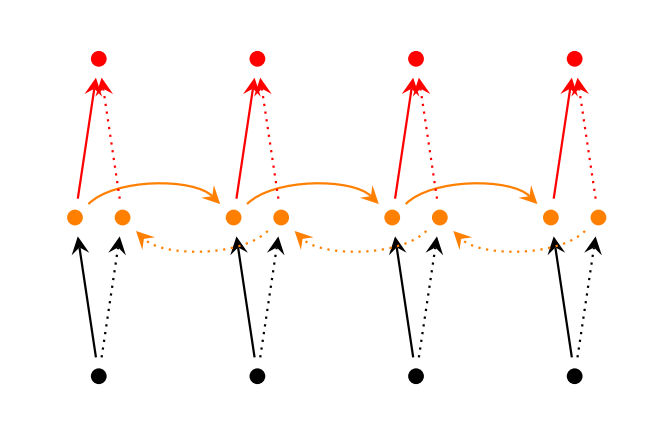
\includegraphics[scale=0.5]{images/bidirectional-rnn}
	\end{figure}
\end{frame}

\section{Wikipedia Dataset}
\begin{frame}{Dataset}
	\begin{itemize}\setlength\itemsep{1em}
		\item For our experiments, the dataset we used is the CoNLL 2010 Shared Task dataset on Wikipedia, one of the benchmark datasets for hedge cue resolution.
		\item The Wikipedia paragraphs were selected based on the hedge cue (called weasels in Wikipedia) tags that were added by the Wikipedia editors, which were subsequently manually annotated.
		\item A sentence is considered uncertain if it contains at least one weasel cue.
	\end{itemize}
	\begin{figure}[htbp]
		\begin{tabular}{|c|c|c|}
			\hline
			\textbf{Certain} & \textbf{Uncertain} & \textbf{Total}\\ 
			\hline
			8627 & 2484 & 11111\\
			\hline
		\end{tabular}
		\caption*{Proportion of class ratios.}
	\end{figure}
\end{frame}
\begin{frame}{Preprocessing}
	We used the following preprocessing of the dataset before feeding it to the NN:
	\begin{itemize}\setlength\itemsep{1em}
		\item Lowercase words.
		\item Removal of XML elements and punctuation.
		\item Tokenization.
		\item Construction of the vocabulary considering only the 27.000 most frequent words.
		%\item Sentences truncation up to \texttt{max\_sentence\_length}.
	\end{itemize}
\end{frame}

\section{The Model}
\begin{frame}{Binary Sentences Classifier Model}
	The model used for the classification task is structured as follows:
	\begin{enumerate}\setlength\itemsep{1em}
		\item Each sentence is represented into a real vector domain.
		\item An embedding layer that converts each word into the corresponding embedding vector; the initial weights are given from GloVe features, scaled in $[-1,1]$ interval, or randomly chosen.
		\item An LSTM or BLSTM layer.
		\item A finally fully-connected neuron with sigmoid as activation function. This last layer takes the scalar probability $P(positive|sentence)$ given at the last timestep output of the LSTM layer.
	\end{enumerate}
\end{frame}
\begin{frame}[shrink=25]
	\frametitle{Binary Sentences Classifier Model}
	\vspace{30px}
	\begin{figure}[htbp]
		
\def\layersep{2cm}

\begin{tikzpicture}[shorten >=1pt,->,draw=black!50, node distance=\layersep]
    \tikzstyle{every pin edge}=[<-,shorten <=1pt]
    \tikzstyle{neuron}=[circle,fill=black!25,minimum size=17pt,inner sep=0pt]
    \tikzstyle{input neuron}=[neuron, fill=black!50];
    \tikzstyle{output neuron}=[neuron, fill=black!50];
    \tikzstyle{hidden neuron}=[neuron, fill=black!50];
    \tikzstyle{project neuron}=[neuron, fill=black!50];
    \tikzstyle{annot} = [text width=4em, text centered]
    \tikzstyle{hoz}=[rotate=-180]  %<--- for labels

    % Draw the input layer nodes
     \node[input neuron, pin=left:"This"] (I-1) at (0,-1) {};
      \node[input neuron, pin=left:"can"] (I-2) at (0,-2) {};
      \node[input neuron, pin=left:"result"] (I-3) at (0,-3) {};
      \node[hoz] (I-4) at (0,-4) {$\dots$};
      \node[input neuron, pin=left:"irritable."] (I-5) at (0,-5) {};


    \foreach \name / \y in {1/1, 2/2, 3/3, 5/5}
            \node[hidden neuron] (E-\name) at (\layersep ,-\y cm) {};
      \node[hoz] (E-4) at (\layersep,-4) {$\dots$};

    \foreach \name / \y in {1/1, 2/2, 3/3, 5/5}
           \node[project neuron] (L-\name) at (\layersep+\layersep,-\y cm) {};
     \node[hoz] (L-4) at (\layersep+\layersep,-4) {$\dots$};


   \node[hidden neuron, right of=L-3] (S) {};

    % Draw the output layer node
    \node[output neuron,pin={[pin edge={->}]right:Final Prediction}, right of=S] (O) {};

    \foreach \current/\next in {1/2, 2/3, 3/4, 4/5}
       {
        \path (L-\current) edge (L-\next);
       }

    % Connect every node in the input layer with every node in the
    % hidden layer.
     	\foreach \source in {1,2,3,5}
           \path (I-\source) edge (E-\source);

    % Connect every node in the hidden layer with the output layer
        \path (S) edge (O);

    \foreach \source in {1,2,3,5}
        \path (E-\source) edge (L-\source);

        \path (L-5) edge (S);


    % Annotate the layers
    \node[annot,above of=E-1, node distance=1cm] (el) {Embedding layer};
    \node[annot,above of=L-1, node distance=1cm] (ll) {LSTM layer};
    \node[annot,above of=S, node distance=1cm] (pl) {Projection Layer};
    \node[annot,above of=O, node distance=1cm] (sl) {Sigmoid};
    \node[annot,left of=el] {Input layer};
    %\node[annot,right of=sl] {Output layer};
\end{tikzpicture}

	\end{figure}
	\begin{itemize}
		\item For BLSTM version we have a Merge layer before Projection layer that receive two input, first relative to the forward propagation and the second relative to the backward propagation.
	\end{itemize}
\end{frame}
\begin{frame}{In-Sentence Cues Detection Model}
	The model used for the in-sentence cues detection task is structured as follows:
	\begin{enumerate}\setlength\itemsep{1em}
		\item Each sentence is represented into a real vector domain.
		\item An embedding layer that converts each word into the corresponding embedding vector; the initial weights are given from GloVe features, scaled in $[-1,1]$ interval, or randomly chosen.
		\item An LSTM or BLSTM layer.
		\item A Merge layer takes the output given at each timestep of the LSTM layer and gives in output the average value.
		\item A finally fully-connected neuron with sigmoid as activation function. This last layer takes the scalar probability given by previous layer.
	\end{enumerate}
\end{frame}
\begin{frame}[shrink=25]
	\frametitle{In-Sentence Cues Detection Model}
	\vspace{30px}
	\begin{figure}[htbp]
		
\def\layersep{2cm}

\begin{tikzpicture}[shorten >=1pt,->,draw=black!50, node distance=\layersep]
    \tikzstyle{every pin edge}=[<-,shorten <=1pt]
    \tikzstyle{neuron}=[circle,fill=black!25,minimum size=17pt,inner sep=0pt]
    \tikzstyle{input neuron}=[neuron, fill=black!50];
    \tikzstyle{output neuron}=[neuron, fill=black!50];
    \tikzstyle{hidden neuron}=[neuron, fill=black!50];
    \tikzstyle{project neuron}=[neuron, fill=black!50];
    \tikzstyle{annot} = [text width=4em, text centered]
    \tikzstyle{hoz}=[rotate=-180]  %<--- for labels

    % Draw the input layer nodes
    % This is the same as writing \foreach \name / \y in {1/1,2/2,3/3,4/4}
    \node[input neuron, pin=left:"This"] (I-1) at (0,-1) {};
      \node[input neuron, pin=left:"can"] (I-2) at (0,-2) {};
      \node[input neuron, pin=left:"result"] (I-3) at (0,-3) {};
      \node[hoz] (I-4) at (0,-4) {$\dots$};
      \node[input neuron, pin=left:"irritable."] (I-5) at (0,-5) {};


    \foreach \name / \y in {1/1, 2/2, 3/3, 5/5}
            \node[hidden neuron] (E-\name) at (\layersep ,-\y cm) {};
      \node[hoz] (E-4) at (\layersep,-4) {$\dots$};

    \foreach \name / \y in {1/1, 2/2, 3/3, 5/5}
           \node[project neuron] (L-\name) at (\layersep+\layersep,-\y cm) {};
     \node[hoz] (L-4) at (\layersep+\layersep,-4) {$\dots$};

   \node[hidden neuron, right of=L-3] (M) {};

   \node[hidden neuron, right of=M] (S) {};

    % Draw the output layer node
    \node[output neuron,pin={[pin edge={->}]right:Final Prediction}, right of=S] (O) {};

    \foreach \current/\next in {1/2,2/3,3/4,4/5}
       {
        \path (L-\current) edge (L-\next);
       }

    % Connect every node in the input layer with every node in the
    % hidden layer.
     	\foreach \source in{1,2,3,5}
           \path (I-\source) edge (E-\source);

    % Connect every node in the hidden layer with the output layer
        \path (S) edge (O);
        \path (M) edge (S);

    \foreach \source in{1,2,3,5}
        \path (E-\source) edge (L-\source);

     \foreach \source in {1,2,3,5}
        \path (L-\source) edge (M);


    % Annotate the layers
    \node[annot,above of=E-1, node distance=1cm] (el) {Embedding layer};
    \node[annot,above of=L-1, node distance=1cm] (ll) {LSTM layer};
    \node[annot,above of=M, node distance=1cm] (ml) {Merge};
    \node[annot,above of=S, node distance=1cm] (pl) {Projection Layer};
    \node[annot,above of=O, node distance=1cm] (sl) {Sigmoid};
    \node[annot,left of=el] {Input layer};
    %\node[annot,right of=sl] {Output layer};
\end{tikzpicture}

	\end{figure}
	\begin{itemize}
		\item For BLSTM version we have another Merge layer, that combines the output of the forward and the backward LSTMs.
	\end{itemize}
\end{frame}
\begin{frame}{Training}
	\begin{itemize}\setlength\itemsep{1em}
		\item To train the model we minimize the binary cross-entropy loss:
		$$\text{Loss} = -\sum_{i=1}^{N}y^{(i)}\log\widetilde{y}^{(i)} + \left(1-y^{(i)}\right)\left(1-\log\widetilde{y}^{(i)}\right)$$
		where $N$ is the number of sentences, $\widetilde{y}^{(i)}$ is the value of the sigmoid layer for the sentence $i$ and $y^{(i)}$ is 1 if the sentence is uncertain, 0 if is certain.
		\item The optimizer used was Adadelta (An Adaptive Learning Rate Method) with Keras default parameters. Other optimizers, like Adam and RMSProp, have been tested for this tasks, but it seems that learning curves didn't change so much.
		\item In addition we used dropout before the (B)LSTM layer, and before the projection layer.
		%\item In addition we used dropout on information that pass between LSTM timesteps, in particular on input and output gates.
	\end{itemize}
\end{frame}

\section{Experimental Settings}
\begin{frame}{Experimental Settings}
	The mini-batch size was fixed to 16 and the results were obtained (for some experiments only) by performing a stratified $k$-fold, with $k=5$, and taking the median value.\\
	\vspace{0.5cm}
	To overcome the unbalanced nature of the dataset, we have extended the training set by replicating uncertain sentences. The minibatches were built simply by putting in half certain and half uncertain sentences.\\
	\vspace{0.5cm}
	The tests were performed by varying the following hyperparameters:
	\begin{itemize}
		\item Number of LSTM layer's cells.
		\item Dropout keep probability.
		\item Embedding weights initialization: with or without GloVe. In the second case, we use the Wikipedia pre-trained 50-dimensional word vectors.
	\end{itemize}
\end{frame}

\section{Results}
\begin{frame}{Results on Sentences Classifier}
	\begin{figure}[htbp]
		\begin{tabular}{|c|c|c|c|c|c|c|}
			%TODO: Group by LSTM units
			\hline
			\textbf{Dropout} & \textbf{LSTM} & \begin{tabular}{@{}c@{}}\textbf{Loss} \\ \textbf{Train}\end{tabular}  & \begin{tabular}{@{}c@{}}\textbf{Loss} \\ \textbf{Test}\end{tabular} & \begin{tabular}{@{}c@{}}\textbf{F-score} \\ \textbf{Train}\end{tabular}  & \begin{tabular}{@{}c@{}}\textbf{F-score} \\ \textbf{Test}\end{tabular} & \textbf{Epoch}\\ 
			\hline
			0.6 & 20 & 0.32 & 0.51 & 0.74 & 0.54 & 39 \\
			0.6 & 25 & 0.29 & 0.50 & 0.76 & 0.55 & 37 \\
			0.6 & 30 & 0.34 & 0.49 & 0.72 & 0.56 & 31 \\
			0.6 & 35 & 0.36 & 0.49 & 0.70 & \textbf{0.57} & 32 \\\hline
			0.7 & 20 & 0.43 & 0.59 & 0.66 & 0.51 & 49 \\
			0.7 & 25 & 0.36 & 0.50 & 0.71 & 0.55 & 47 \\
			0.7 & 30 & 0.35 & 0.54 & 0.71 & 0.53 & 47 \\
			0.7 & 35 & 0.38 & 0.52 & 0.69 & \textbf{0.55} & 50 \\
			\hline
		\end{tabular}
		\caption*{Results on unidirectional model with GloVe}
	\end{figure}
\end{frame}
\begin{frame}{Comments}
	\begin{itemize}\setlength\itemsep{1em}
		\item With dropout 0.6 the model reaches the best performance in few epochs, while the number of LSTM units didn't influence very much.		
		\item Changing the dropout keep probability doesn't improve much the $F$-score, but the model needs much epochs to converge.
		\item The best results of $F$-score is obtained with 35 LSTM units.
	\end{itemize}
\end{frame}
\begin{frame}{Learning Curves on Unidirectional Model}
	\begin{tikzpicture}
	\begin{axis}[%
	width=1\textwidth,
	height=0.65\textwidth,
	xmin=1, xmax=50,
	ymin=0.3, ymax=1,
	xtick={0,10,...,50},
	ytick={0,0.1,...,1},
	%minor x tick num= 1,
	%minor y tick num= 1,
	axis x line=bottom,
	axis y line=left,
	%axis x discontinuity=crunch,
	xlabel={Epochs}, ylabel={$F$-score}, title={},
	axis on top=true, clip=false
	]
	\addplot [smooth, color=blue] coordinates {
		(1, 0.432449)
		(2, 0.435576)
		(3, 0.438315)
		(4, 0.440506)
		(5, 0.442671)
		(6, 0.448247)
		(7, 0.450336)
		(8, 0.454786)
		(9, 0.458624)
		(10, 0.463905)
		(11, 0.472802)
		(12, 0.475094)
		(13, 0.48342)
		(14, 0.491634)
		(15, 0.498842)
		(16, 0.510398)
		(17, 0.526418)
		(18, 0.533691)
		(19, 0.543522)
		(20, 0.55506)
		(21, 0.576248)
		(22, 0.605361)
		(23, 0.610295)
		(24, 0.612736)
		(25, 0.640748)
		(26, 0.647498)
		(27, 0.658239)
		(28, 0.669953)
		(29, 0.679954)
		(30, 0.684149)
		(31, 0.697291)
		(32, 0.700685)
		(33, 0.706853)
		(34, 0.718164)
		(35, 0.724754)
		(36, 0.727372)
		(37, 0.742686)
		(38, 0.749401)
		(39, 0.757805)
		(40, 0.764203)
		(41, 0.779222)
		(42, 0.794207)
		(43, 0.797633)
		(44, 0.804302)
		(45, 0.811213)
		(46, 0.822894)
		(47, 0.82841)
		(48, 0.834853)
		(49, 0.842856)
		(50, 0.848163)
	};
	\addplot [smooth, color=red] coordinates {
		(1, 0.416081)
		(2, 0.413257)
		(3, 0.418655)
		(4, 0.419146)
		(5, 0.422492)
		(6, 0.426181)
		(7, 0.427512)
		(8, 0.429425)
		(9, 0.431328)
		(10, 0.435746)
		(11, 0.44513)
		(12, 0.445041)
		(13, 0.448339)
		(14, 0.452703)
		(15, 0.458701)
		(16, 0.464288)
		(17, 0.469482)
		(18, 0.477558)
		(19, 0.478662)
		(20, 0.490901)
		(21, 0.506788)
		(22, 0.524113)
		(23, 0.530811)
		(24, 0.530392)
		(25, 0.541655)
		(26, 0.543793)
		(27, 0.5443)
		(28, 0.554995)
		(29, 0.560952)
		(30, 0.557281)
		(31, 0.566309)
		(32, 0.567542)
		(33, 0.567138)
		(34, 0.56818)
		(35, 0.563531)
		(36, 0.558475)
		(37, 0.555915)
		(38, 0.557478)
		(39, 0.552872)
		(40, 0.551989)
		(41, 0.546153)
		(42, 0.547786)
		(43, 0.547071)
		(44, 0.543775)
		(45, 0.538705)
		(46, 0.527589)
		(47, 0.525248)
		(48, 0.521054)
		(49, 0.516076)
		(50, 0.52112)
	};
	\addlegendentry{Train}
	\addlegendentry{Test}
	\end{axis}
	\end{tikzpicture}
	\begin{center}
		Results with dropout 0.6, best $F$-score 0.57 at epoch 32.
	\end{center}
\end{frame}
\begin{frame}{Learning Curves on Unidirectional Model}
	\begin{tikzpicture}
		\begin{axis}[%
		width=1\textwidth,
		height=0.65\textwidth,
		xmin=1, xmax=50,
		ymin=0, ymax=0.8,
		xtick={0,10,...,50},
		ytick={0,0.1,...,0.8},
		%minor x tick num= 1,
		%minor y tick num= 1,
		axis x line=bottom,
		axis y line=left,
		%axis x discontinuity=crunch,
		xlabel={Epochs}, ylabel={Loss}, title={},
		axis on top=true, clip=false
		]
		\addplot [smooth, color=blue] coordinates {
			(1, 0.703353)
			(2, 0.71473)
			(3, 0.709559)
			(4, 0.713786)
			(5, 0.712943)
			(6, 0.701872)
			(7, 0.693549)
			(8, 0.683538)
			(9, 0.669548)
			(10, 0.645073)
			(11, 0.62499)
			(12, 0.620852)
			(13, 0.611292)
			(14, 0.598629)
			(15, 0.592278)
			(16, 0.579367)
			(17, 0.563401)
			(18, 0.562355)
			(19, 0.558014)
			(20, 0.54493)
			(21, 0.514857)
			(22, 0.473622)
			(23, 0.471563)
			(24, 0.477688)
			(25, 0.433763)
			(26, 0.433562)
			(27, 0.419151)
			(28, 0.402275)
			(29, 0.389357)
			(30, 0.387116)
			(31, 0.359439)
			(32, 0.35527)
			(33, 0.347825)
			(34, 0.330842)
			(35, 0.319338)
			(36, 0.319346)
			(37, 0.293432)
			(38, 0.288731)
			(39, 0.281516)
			(40, 0.274789)
			(41, 0.251402)
			(42, 0.233962)
			(43, 0.230923)
			(44, 0.225959)
			(45, 0.223471)
			(46, 0.205092)
			(47, 0.197124)
			(48, 0.188349)
			(49, 0.178808)
			(50, 0.171163)
		};
		\addplot [smooth, color=red] coordinates {
			(1, 0.703682)
			(2, 0.715624)
			(3, 0.710498)
			(4, 0.715678)
			(5, 0.715794)
			(6, 0.705948)
			(7, 0.699425)
			(8, 0.692231)
			(9, 0.680194)
			(10, 0.658328)
			(11, 0.640737)
			(12, 0.639723)
			(13, 0.634652)
			(14, 0.626652)
			(15, 0.625403)
			(16, 0.617889)
			(17, 0.608569)
			(18, 0.614124)
			(19, 0.614302)
			(20, 0.606375)
			(21, 0.579672)
			(22, 0.541123)
			(23, 0.54205)
			(24, 0.553103)
			(25, 0.510049)
			(26, 0.516496)
			(27, 0.508631)
			(28, 0.498903)
			(29, 0.492935)
			(30, 0.502326)
			(31, 0.483212)
			(32, 0.488398)
			(33, 0.491479)
			(34, 0.485577)
			(35, 0.486231)
			(36, 0.499699)
			(37, 0.484544)
			(38, 0.491666)
			(39, 0.496815)
			(40, 0.5061)
			(41, 0.494402)
			(42, 0.489007)
			(43, 0.500123)
			(44, 0.510555)
			(45, 0.520335)
			(46, 0.515869)
			(47, 0.518797)
			(48, 0.528623)
			(49, 0.53345)
			(50, 0.533377)
		};
		\addlegendentry{Train}
		\addlegendentry{Test}
		\end{axis}
	\end{tikzpicture}
	\begin{center}
		Results with dropout 0.6, and 35 LSTM units.
	\end{center}
\end{frame}

\begin{frame}{Results on Sentences Classifier (BLSTM)}
	\begin{table}%[htbp]
		\resizebox{0.7\textwidth}{!}{%
			\begin{tabular}{|c|c|c|c|c|c|c|c|}
				\hline
				\textbf{GloVe} & \textbf{Dropout} & \textbf{LSTM} & \begin{tabular}{@{}c@{}}\textbf{Loss} \\ \textbf{Train}\end{tabular}  & \begin{tabular}{@{}c@{}}\textbf{Loss} \\ \textbf{Test}\end{tabular} & \begin{tabular}{@{}c@{}}\textbf{F-score} \\ \textbf{Train}\end{tabular}  & \begin{tabular}{@{}c@{}}\textbf{F-score} \\ \textbf{Test}\end{tabular} & \textbf{Epoch}\\ 
				\hline
				yes & 1 & 20 & 0.19 & 0.43 & 0.82 & 0.57 & 8 \\
				yes & 0.6 & 20 & 0.30 & 0.52 & 0.75 & \textbf{0.59} & 42 \\
				no & 0.6 & 20 & 0.15 & 0.65 & 0.87 & 0.47 & 31 \\\hline
				yes & 0.6 & 25 & 0.30 & 0.43 & 0.72 & \textbf{0.59} & 5 \\
				no & 0.6 & 25 & 0.29 & 0.53 & 0.76 & 0.52 & 19 \\\hline
				yes & 0.6 & 30 & 0.23 & 0.47 & 0.79 & \textbf{0.58} & 7 \\
				no & 0.6 & 30 & 0.30 & 0.55 & 0.76 & 0.53 & 19 \\\hline
				yes & 0.6 & 35 & 0.23 & 0.48 & 0.79 & \textbf{0.59} & 7 \\
				no & 0.6 & 35 & 0.27 & 0.55 & 0.78 & 0.54 & 21 \\\hline
				yes & 0.7 & 10 & 0.35 & 0.49 & 0.72 & \textbf{0.58} & 50 \\
				yes & 0.7 & 15 & 0.40 & 0.54 & 0.67 & 0.56 & 50 \\\hline
				yes & 1 & 20 & 0.33 & 0.42 & 0.69 & 0.58 & 4 \\
				yes & 0.7 & 20 & 0.23 & 0.62 & 0.81 & \textbf{0.58} & 4 \\
				no & 0.7 & 20 & 0.33 & 0.42 & 0.69 & 0.47 & 40 \\\hline
				yes & 0.7 & 25 & 0.29 & 0.44 & 0.74 & \textbf{0.60} & 6 \\
				no & 0.7 & 25 & 0.25 & 0.60 & 0.79 & 0.49 & 38 \\\hline
				yes & 0.7 & 30 & 0.29 & 0.45 & 0.73 & \textbf{0.57} & 5 \\
				no & 0.7 & 30 & 0.30 & 0.60 & 0.76 & 0.51 & 33 \\\hline
				yes & 0.7 & 35 & 0.29 & 0.45 & 0.74 & \textbf{0.58} & 5 \\
				no & 0.7 & 35 & 0.27 & 0.59 & 0.78 & 0.51 & 35 \\\hline
			\end{tabular}}
		\caption*{Results on bidirectional model}
	\end{table}
\end{frame}
\begin{frame}{Comments}
	\begin{itemize}
		\item The number of LSTM units affect much on the network learning speed, in case we have the GloVe features.
		\item By increasing the number of LSTM units, the network reaches maximum performance in a few epochs.
		\item With the same number of LSTM units the network requires a greater number of epochs to reach the maximum performance.
		\item BLSTM networks generally performs better than simple LSTM networks, with equal number of units for each direction, because the output layer get information from past and future states.
		\item As in the unidirectional model, the dropout doesn't affect much on performance.
		\item For models that converge very quickly, we tried to execute them without GloVe features, and we have noticed that, further the number of units LSTM, also GloVe features affecting the way of learning network, like the speed of learning and accuracy in the learning phase.
	\end{itemize}
\end{frame}

%-----------------------------------------------------------

\begin{frame}{Learning Curves on Bidirectional Model}
	\begin{tikzpicture}
	\begin{axis}[%
	width=1\textwidth,
	height=0.65\textwidth,
	xmin=1, xmax=50,
	ymin=0.3, ymax=1,
	xtick={0,10,...,50},
	ytick={0,0.1,...,1},
	%minor x tick num= 1,
	%minor y tick num= 1,
	axis x line=bottom,
	axis y line=left,
	%axis x discontinuity=crunch,
	xlabel={Epochs}, ylabel={$F$-score}, title={},
	axis on top=true, clip=false
	]
	\addplot [smooth, color=blue] coordinates {
		(1, 0.368923)
		(2, 0.402085)
		(3, 0.417042)
		(4, 0.4326)
		(5, 0.433376)
		(6, 0.437836)
		(7, 0.441129)
		(8, 0.443371)
		(9, 0.448053)
		(10, 0.452445)
		(11, 0.454696)
		(12, 0.456772)
		(13, 0.45565)
		(14, 0.457471)
		(15, 0.463994)
		(16, 0.465345)
		(17, 0.468108)
		(18, 0.471503)
		(19, 0.477514)
		(20, 0.481386)
		(21, 0.48639)
		(22, 0.493295)
		(23, 0.502071)
		(24, 0.507249)
		(25, 0.517753)
		(26, 0.529737)
		(27, 0.532342)
		(28, 0.543285)
		(29, 0.559462)
		(30, 0.571395)
		(31, 0.583365)
		(32, 0.596418)
		(33, 0.607429)
		(34, 0.615933)
		(35, 0.620996)
		(36, 0.629353)
		(37, 0.639736)
		(38, 0.645296)
		(39, 0.652108)
		(40, 0.66739)
		(41, 0.673033)
		(42, 0.677121)
		(43, 0.682385)
		(44, 0.68439)
		(45, 0.699714)
		(46, 0.69829)
		(47, 0.707578)
		(48, 0.710054)
		(49, 0.715757)
		(50, 0.716177)
	};
	\addplot [smooth, color=red] coordinates {
		(1, 0.349328)
		(2, 0.391992)
		(3, 0.402231)
		(4, 0.41308)
		(5, 0.415757)
		(6, 0.421338)
		(7, 0.428224)
		(8, 0.431667)
		(9, 0.436866)
		(10, 0.440027)
		(11, 0.447902)
		(12, 0.453192)
		(13, 0.45045)
		(14, 0.450536)
		(15, 0.45275)
		(16, 0.453943)
		(17, 0.456105)
		(18, 0.457432)
		(19, 0.458714)
		(20, 0.461009)
		(21, 0.463168)
		(22, 0.470321)
		(23, 0.475931)
		(24, 0.481967)
		(25, 0.484247)
		(26, 0.492116)
		(27, 0.494629)
		(28, 0.501622)
		(29, 0.507617)
		(30, 0.51565)
		(31, 0.51933)
		(32, 0.530331)
		(33, 0.529587)
		(34, 0.541376)
		(35, 0.549278)
		(36, 0.555189)
		(37, 0.556464)
		(38, 0.559567)
		(39, 0.563512)
		(40, 0.563289)
		(41, 0.565275)
		(42, 0.566904)
		(43, 0.569666)
		(44, 0.56825)
		(45, 0.572672)
		(46, 0.572439)
		(47, 0.57443)
		(48, 0.578224)
		(49, 0.574952)
		(50, 0.576389)
	};
	\addlegendentry{Train}
	\addlegendentry{Test}
	\end{axis}
	\end{tikzpicture}
	\begin{center}
		Results with dropout 0.7, 10 LSTM units, and best $F$-score 0.58 at epoch 50.
	\end{center}
\end{frame}
\begin{frame}{Learning Curves on Bidirectional Model}
	\begin{tikzpicture}
	\begin{axis}[%
	width=1\textwidth,
	height=0.65\textwidth,
	xmin=1, xmax=50,
	ymin=0, ymax=0.8,
	xtick={0,10,...,50},
	ytick={0,0.1,...,0.8},
	%minor x tick num= 1,
	%minor y tick num= 1,
	axis x line=bottom,
	axis y line=left,
	%axis x discontinuity=crunch,
	xlabel={Epochs}, ylabel={Loss}, title={},
	axis on top=true, clip=false
	]
	\addplot [smooth, color=blue] coordinates {
		(1, 0.689759)
		(2, 0.68709)
		(3, 0.68852)
		(4, 0.684174)
		(5, 0.682282)
		(6, 0.678238)
		(7, 0.673104)
		(8, 0.669467)
		(9, 0.667272)
		(10, 0.655739)
		(11, 0.656439)
		(12, 0.653454)
		(13, 0.659476)
		(14, 0.655701)
		(15, 0.644783)
		(16, 0.646024)
		(17, 0.643061)
		(18, 0.634579)
		(19, 0.626568)
		(20, 0.622933)
		(21, 0.612631)
		(22, 0.611594)
		(23, 0.601052)
		(24, 0.601959)
		(25, 0.583295)
		(26, 0.565942)
		(27, 0.572124)
		(28, 0.564568)
		(29, 0.547522)
		(30, 0.5266)
		(31, 0.518291)
		(32, 0.503161)
		(33, 0.480788)
		(34, 0.475715)
		(35, 0.471789)
		(36, 0.460783)
		(37, 0.440411)
		(38, 0.435529)
		(39, 0.428618)
		(40, 0.405518)
		(41, 0.401263)
		(42, 0.39644)
		(43, 0.390142)
		(44, 0.389204)
		(45, 0.366618)
		(46, 0.371489)
		(47, 0.360006)
		(48, 0.358631)
		(49, 0.347239)
		(50, 0.349156)
	};
	\addplot [smooth, color=red] coordinates {
		(1, 0.690666)
		(2, 0.688246)
		(3, 0.690092)
		(4, 0.686027)
		(5, 0.684562)
		(6, 0.68088)
		(7, 0.676402)
		(8, 0.673517)
		(9, 0.67199)
		(10, 0.661595)
		(11, 0.663271)
		(12, 0.661444)
		(13, 0.66777)
		(14, 0.66623)
		(15, 0.656942)
		(16, 0.659387)
		(17, 0.658576)
		(18, 0.65194)
		(19, 0.647235)
		(20, 0.645724)
		(21, 0.639005)
		(22, 0.640979)
		(23, 0.634765)
		(24, 0.639736)
		(25, 0.625396)
		(26, 0.614238)
		(27, 0.623052)
		(28, 0.619089)
		(29, 0.605347)
		(30, 0.588809)
		(31, 0.583972)
		(32, 0.573738)
		(33, 0.555527)
		(34, 0.553975)
		(35, 0.550548)
		(36, 0.543351)
		(37, 0.527819)
		(38, 0.527017)
		(39, 0.522959)
		(40, 0.505415)
		(41, 0.506077)
		(42, 0.50487)
		(43, 0.503796)
		(44, 0.505951)
		(45, 0.490586)
		(46, 0.500554)
		(47, 0.494132)
		(48, 0.497903)
		(49, 0.4888)
		(50, 0.496667)
	};
	\addlegendentry{Train}
	\addlegendentry{Test}
	\end{axis}
	\end{tikzpicture}
	\begin{center}
		Results with dropout 0.7 and 10 LSTM units
	\end{center}
\end{frame}

%-----------------------------------------------------------
\begin{frame}{Learning Curves on Bidirectional Model}
	\begin{tikzpicture}
	\begin{axis}[%
	width=1\textwidth,
	height=0.65\textwidth,
	xmin=1, xmax=70,
	ymin=0.3, ymax=1,
	xtick={0,10,...,70},
	ytick={0,0.1,...,1},
	%minor x tick num= 1,
	%minor y tick num= 1,
	axis x line=bottom,
	axis y line=left,
	%axis x discontinuity=crunch,
	xlabel={Epochs}, ylabel={$F$-score}, title={},
	axis on top=true, clip=false
	]
	\addplot [smooth, color=blue] coordinates {
		(1, 0.4175)
		(2, 0.4279)
		(3, 0.4319)
		(4, 0.4398)
		(5, 0.4416)
		(6, 0.4453)
		(7, 0.4509)
		(8, 0.452)
		(9, 0.4533)
		(10, 0.4581)
		(11, 0.4601)
		(12, 0.4682)
		(13, 0.4716)
		(14, 0.4774)
		(15, 0.4889)
		(16, 0.4972)
		(17, 0.5039)
		(18, 0.5142)
		(19, 0.526)
		(20, 0.5421)
		(21, 0.5456)
		(22, 0.5543)
		(23, 0.5749)
		(24, 0.5869)
		(25, 0.5914)
		(26, 0.6017)
		(27, 0.6093)
		(28, 0.6303)
		(29, 0.6349)
		(30, 0.6447)
		(31, 0.6548)
		(32, 0.6617)
		(33, 0.6676)
		(34, 0.685)
		(35, 0.6919)
		(36, 0.6979)
		(37, 0.7087)
		(38, 0.7096)
		(39, 0.7235)
		(40, 0.7282)
		(41, 0.7405)
		(42, 0.7454)
		(43, 0.7525)
		(44, 0.7551)
		(45, 0.7628)
		(46, 0.7726)
		(47, 0.7833)
		(48, 0.7911)
		(49, 0.7994)
		(50, 0.7993)
		(51, 0.8098)
		(52, 0.8267)
		(53, 0.8304)
		(54, 0.8355)
		(55, 0.8378)
		(56, 0.8461)
		(57, 0.8588)
		(58, 0.8604)
		(59, 0.8663)
		(60, 0.8681)
		(61, 0.8748)
		(62, 0.8868)
		(63, 0.8755)
		(64, 0.8906)
		(65, 0.8958)
		(66, 0.8956)
		(67, 0.9006)
		(68, 0.9063)
		(69, 0.9082)
		(70, 0.9174)
	};
	\addplot [smooth, color=red] coordinates {
		(1, 0.4109)
		(2, 0.419)
		(3, 0.4242)
		(4, 0.4284)
		(5, 0.4308)
		(6, 0.4384)
		(7, 0.4439)
		(8, 0.4492)
		(9, 0.4476)
		(10, 0.45)
		(11, 0.4506)
		(12, 0.454)
		(13, 0.4558)
		(14, 0.4636)
		(15, 0.4695)
		(16, 0.4691)
		(17, 0.4779)
		(18, 0.4836)
		(19, 0.4883)
		(20, 0.4953)
		(21, 0.5014)
		(22, 0.5089)
		(23, 0.5124)
		(24, 0.5214)
		(25, 0.5227)
		(26, 0.524)
		(27, 0.5309)
		(28, 0.5354)
		(29, 0.5458)
		(30, 0.5507)
		(31, 0.5601)
		(32, 0.5638)
		(33, 0.5665)
		(34, 0.5749)
		(35, 0.5784)
		(36, 0.5807)
		(37, 0.5773)
		(38, 0.5802)
		(39, 0.5831)
		(40, 0.586)
		(41, 0.5877)
		(42, 0.5897)
		(43, 0.5842)
		(44, 0.5784)
		(45, 0.5742)
		(46, 0.5729)
		(47, 0.574)
		(48, 0.5724)
		(49, 0.5664)
		(50, 0.5796)
		(51, 0.5634)
		(52, 0.5541)
		(53, 0.5534)
		(54, 0.5558)
		(55, 0.5573)
		(56, 0.5546)
		(57, 0.5571)
		(58, 0.5505)
		(59, 0.5531)
		(60, 0.5555)
		(61, 0.5512)
		(62, 0.544)
		(63, 0.5515)
		(64, 0.5344)
		(65, 0.5373)
		(66, 0.54)
		(67, 0.5387)
		(68, 0.5352)
		(69, 0.5373)
		(70, 0.5287)
	};
	\addlegendentry{Train}
	\addlegendentry{Test}
	\end{axis}
	\end{tikzpicture}
	\begin{center}
		Results with dropout 0.6, 20 LSTM units, and best $F$-score 0.57 at epoch 42
	\end{center}
\end{frame}
\begin{frame}{Learning Curves on Bidirectional Model}
	\begin{tikzpicture}
	\begin{axis}[%
	width=1\textwidth,
	height=0.65\textwidth,
	xmin=1, xmax=70,
	ymin=0, ymax=0.8,
	xtick={0,10,...,70},
	ytick={0,0.1,...,0.8},
	%minor x tick num= 1,
	%minor y tick num= 1,
	axis x line=bottom,
	axis y line=left,
	%axis x discontinuity=crunch,
	xlabel={Epochs}, ylabel={Loss}, title={},
	axis on top=true, clip=false
	]
	\addplot [smooth, color=blue] coordinates {
		(1, 0.695356)
		(2, 0.693097)
		(3, 0.696722)
		(4, 0.683924)
		(5, 0.677347)
		(6, 0.673967)
		(7, 0.660616)
		(8, 0.658674)
		(9, 0.654551)
		(10, 0.641751)
		(11, 0.639625)
		(12, 0.631933)
		(13, 0.627436)
		(14, 0.622976)
		(15, 0.613711)
		(16, 0.606705)
		(17, 0.600808)
		(18, 0.587483)
		(19, 0.578672)
		(20, 0.557306)
		(21, 0.561472)
		(22, 0.550003)
		(23, 0.522051)
		(24, 0.508629)
		(25, 0.504642)
		(26, 0.493575)
		(27, 0.479269)
		(28, 0.453084)
		(29, 0.449302)
		(30, 0.429137)
		(31, 0.414494)
		(32, 0.403248)
		(33, 0.399193)
		(34, 0.378231)
		(35, 0.371182)
		(36, 0.358944)
		(37, 0.346938)
		(38, 0.342753)
		(39, 0.322659)
		(40, 0.319939)
		(41, 0.303791)
		(42, 0.300925)
		(43, 0.294813)
		(44, 0.290642)
		(45, 0.277828)
		(46, 0.271464)
		(47, 0.259901)
		(48, 0.252903)
		(49, 0.242509)
		(50, 0.245228)
		(51, 0.228291)
		(52, 0.203732)
		(53, 0.200391)
		(54, 0.193314)
		(55, 0.197509)
		(56, 0.188945)
		(57, 0.171652)
		(58, 0.171723)
		(59, 0.162586)
		(60, 0.162188)
		(61, 0.150975)
		(62, 0.135857)
		(63, 0.15218)
		(64, 0.12948)
		(65, 0.125723)
		(66, 0.128643)
		(67, 0.120186)
		(68, 0.112147)
		(69, 0.112108)
		(70, 0.0994469)
	};
	\addplot [smooth, color=red] coordinates {
		(1, 0.695657)
		(2, 0.693975)
		(3, 0.69805)
		(4, 0.686042)
		(5, 0.680006)
		(6, 0.677387)
		(7, 0.664939)
		(8, 0.664116)
		(9, 0.661685)
		(10, 0.651825)
		(11, 0.651275)
		(12, 0.648584)
		(13, 0.645931)
		(14, 0.646534)
		(15, 0.641926)
		(16, 0.639137)
		(17, 0.637216)
		(18, 0.629312)
		(19, 0.626637)
		(20, 0.611075)
		(21, 0.620051)
		(22, 0.613747)
		(23, 0.593274)
		(24, 0.586364)
		(25, 0.586699)
		(26, 0.581873)
		(27, 0.571356)
		(28, 0.553889)
		(29, 0.555358)
		(30, 0.540069)
		(31, 0.533192)
		(32, 0.530553)
		(33, 0.533431)
		(34, 0.519279)
		(35, 0.521028)
		(36, 0.517929)
		(37, 0.516411)
		(38, 0.519322)
		(39, 0.50935)
		(40, 0.51686)
		(41, 0.510501)
		(42, 0.518265)
		(43, 0.523762)
		(44, 0.523898)
		(45, 0.527079)
		(46, 0.53173)
		(47, 0.530826)
		(48, 0.538403)
		(49, 0.539289)
		(50, 0.557643)
		(51, 0.55822)
		(52, 0.549789)
		(53, 0.553841)
		(54, 0.555772)
		(55, 0.572469)
		(56, 0.582669)
		(57, 0.581301)
		(58, 0.593478)
		(59, 0.599317)
		(60, 0.602411)
		(61, 0.605296)
		(62, 0.609174)
		(63, 0.628246)
		(64, 0.625454)
		(65, 0.62701)
		(66, 0.642637)
		(67, 0.642923)
		(68, 0.653434)
		(69, 0.668434)
		(70, 0.670116)
	};
	\addlegendentry{Train}
	\addlegendentry{Test}
	\end{axis}
	\end{tikzpicture}
	\begin{center}
		Results with dropout 0.6 and 20 LSTM units
	\end{center}
\end{frame}
\begin{frame}{Learning Curves with and without GloVe}
	\begin{tikzpicture}
	\begin{axis}[%
	width=1\textwidth,
	height=0.65\textwidth,
	xmin=1, xmax=50,
	ymin=0, ymax=0.8,
	xtick={0,10,...,50},
	ytick={0,0.1,...,0.8},
	%minor x tick num= 1,
	%minor y tick num= 1,
	axis x line=bottom,
	axis y line=left,
	%axis x discontinuity=crunch,
	xlabel={Epochs}, ylabel={$F$-score (test)}, title={},
	axis on top=true, clip=false
	]
	\addplot [smooth, color=blue] coordinates {
		(1, 0.4109)
		(2, 0.419)
		(3, 0.4242)
		(4, 0.4284)
		(5, 0.4308)
		(6, 0.4384)
		(7, 0.4439)
		(8, 0.4492)
		(9, 0.4476)
		(10, 0.45)
		(11, 0.4506)
		(12, 0.454)
		(13, 0.4558)
		(14, 0.4636)
		(15, 0.4695)
		(16, 0.4691)
		(17, 0.4779)
		(18, 0.4836)
		(19, 0.4883)
		(20, 0.4953)
		(21, 0.5014)
		(22, 0.5089)
		(23, 0.5124)
		(24, 0.5214)
		(25, 0.5227)
		(26, 0.524)
		(27, 0.5309)
		(28, 0.5354)
		(29, 0.5458)
		(30, 0.5507)
		(31, 0.5601)
		(32, 0.5638)
		(33, 0.5665)
		(34, 0.5749)
		(35, 0.5784)
		(36, 0.5807)
		(37, 0.5773)
		(38, 0.5802)
		(39, 0.5831)
		(40, 0.586)
		(41, 0.5877)
		(42, 0.5897)
		(43, 0.5842)
		(44, 0.5784)
		(45, 0.5742)
		(46, 0.5729)
		(47, 0.574)
		(48, 0.5724)
		(49, 0.5664)
		(50, 0.5796)
	};
	\addplot [smooth, color=red] coordinates {
		(1, 0.00360036)
		(2, 0.0626702)
		(3, 0.286839)
		(4, 0.329944)
		(5, 0.38521)
		(6, 0.42319)
		(7, 0.439895)
		(8, 0.44809)
		(9, 0.46179)
		(10, 0.453653)
		(11, 0.455213)
		(12, 0.466221)
		(13, 0.467746)
		(14, 0.479184)
		(15, 0.477447)
		(16, 0.478356)
		(17, 0.485431)
		(18, 0.486758)
		(19, 0.489175)
		(20, 0.488948)
		(21, 0.495294)
		(22, 0.494186)
		(23, 0.497303)
		(24, 0.494437)
		(25, 0.492222)
		(26, 0.479542)
		(27, 0.479909)
		(28, 0.477304)
		(29, 0.475068)
		(30, 0.466769)
		(31, 0.469544)
		(32, 0.461919)
		(33, 0.461824)
		(34, 0.455538)
		(35, 0.437288)
		(36, 0.452891)
		(37, 0.432485)
		(38, 0.433464)
		(39, 0.430031)
		(40, 0.427954)
		(41, 0.431826)
		(42, 0.430231)
		(43, 0.426202)
		(44, 0.430316)
		(45, 0.426621)
		(46, 0.429875)
		(47, 0.42949)
		(48, 0.42644)
		(49, 0.423066)
		(50, 0.42349)
	};
	\addlegendentry{with GloVe}
	\addlegendentry{w/o GloVe}
	\end{axis}
	\end{tikzpicture}
	\begin{center}
		Results with dropout 0.6, 20 LSTM units, and best $F$-score 0.57 at epoch 42
	\end{center}
\end{frame}
\begin{frame}{Results for In-Sentence Cue Detection}
	\begin{table}%[htbp]
		\resizebox{0.75\textwidth}{!}{%
			\begin{tabular}{|c|c|c|c|c|}
				\hline
				\textbf{Best Cue Threshold} & \textbf{Accuracy} & \textbf{Precision} & \textbf{Recall} & \textbf{F-score} \\
				\hline
				0.31 & 0.89 & 0.19 & 0.59 & 0.28\\
				\hline
			\end{tabular}}
		\caption*{Unidirectional model with $F$-score 0.54, dropout 0.6, LSTM units 15}
	\end{table}
	\begin{table}%[htbp]
		\resizebox{0.75\textwidth}{!}{%
			\begin{tabular}{|c|c|c|c|c|}
				\hline
				\textbf{Best Cue Threshold} & \textbf{Accuracy} & \textbf{Precision} & \textbf{Recall} & \textbf{F-score} \\
				\hline
				0.46 & 0.91 & 0.29 & 0.36 & 0.32\\
				\hline
			\end{tabular}}
			\caption*{Bidirectional model with $F$-score 0.56, dropout 0.6, LSTM units 10}
	\end{table}
	Bidirectional model performs much better for in-sentence cue detections, maybe with backward passes it collect some important features on syntactic information.
\end{frame}
\begin{frame}{Results for In-Sentence Cue Detection}
	\begin{figure}[htbp]
		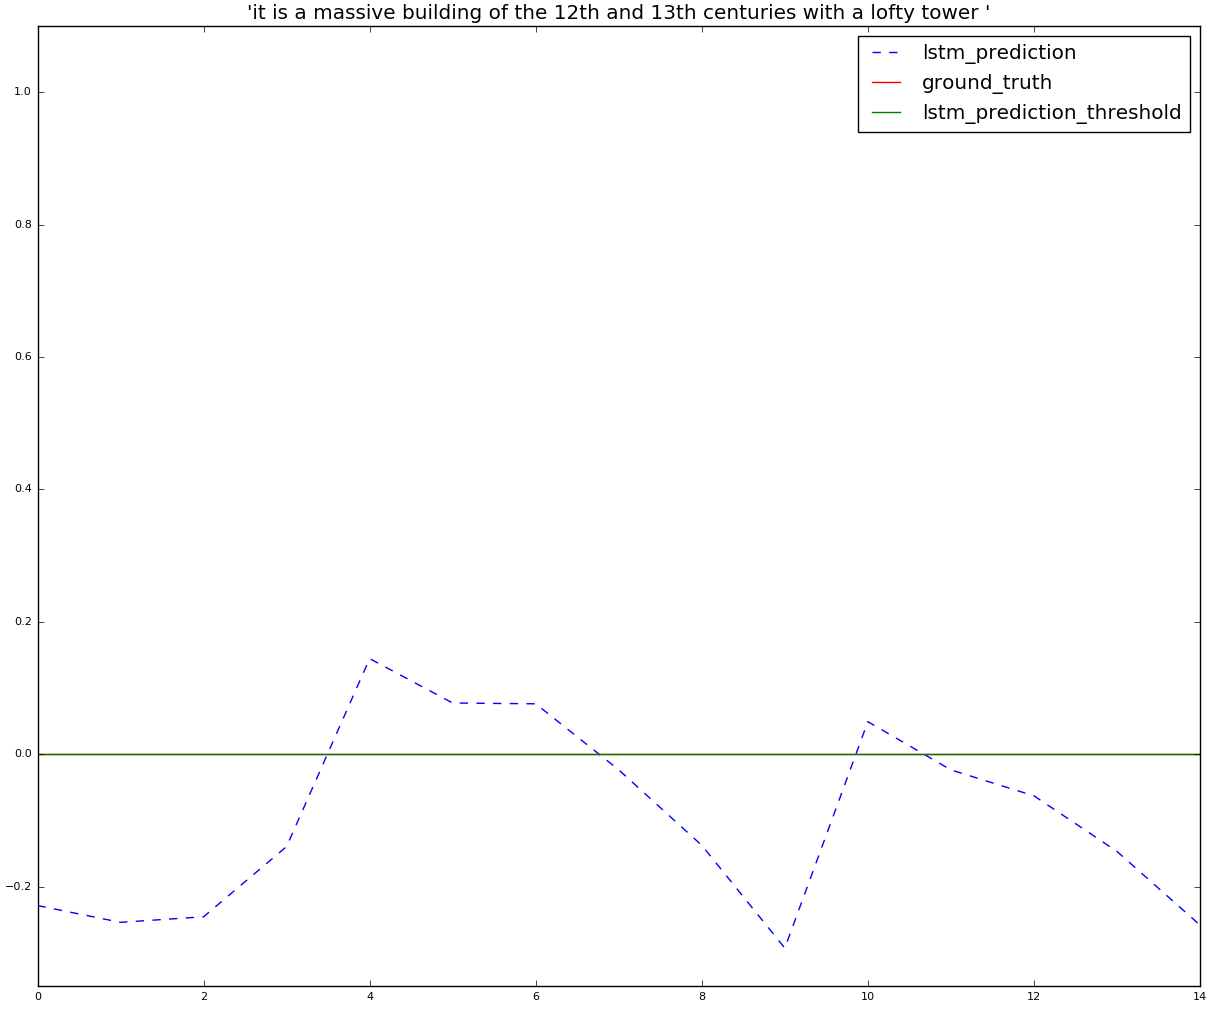
\includegraphics[scale=0.3]{images/task2_1dir/27_type0}
	\end{figure}
\end{frame}
\begin{frame}{Results for In-Sentence Cue Detection}
	\begin{figure}[htbp]
		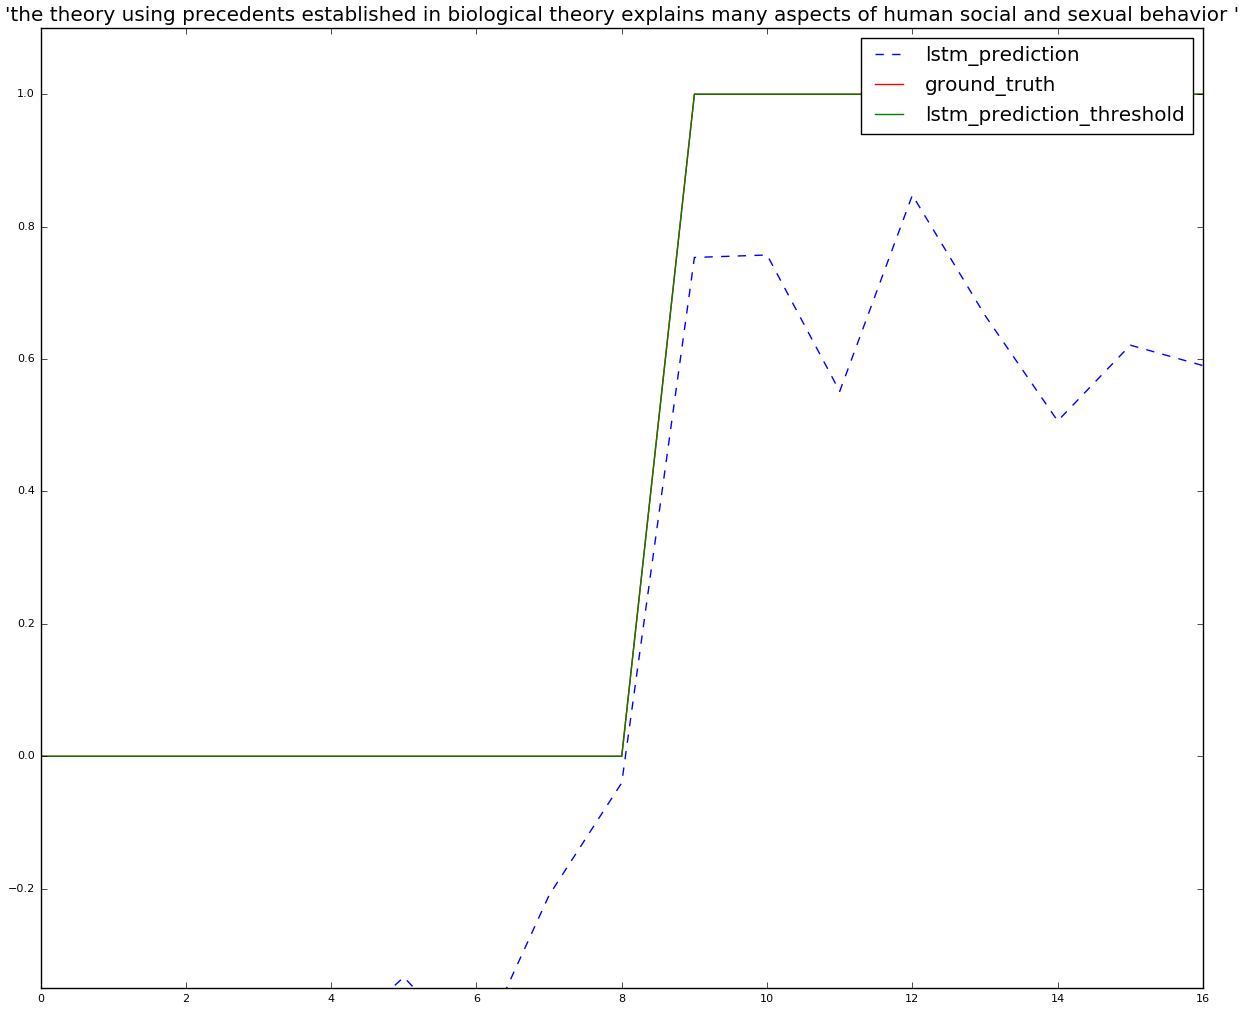
\includegraphics[scale=0.3]{images/task2_1dir/25_type1}
	\end{figure}
\end{frame}
\begin{frame}{Results for In-Sentence Cue Detection}
	\begin{figure}[htbp]
		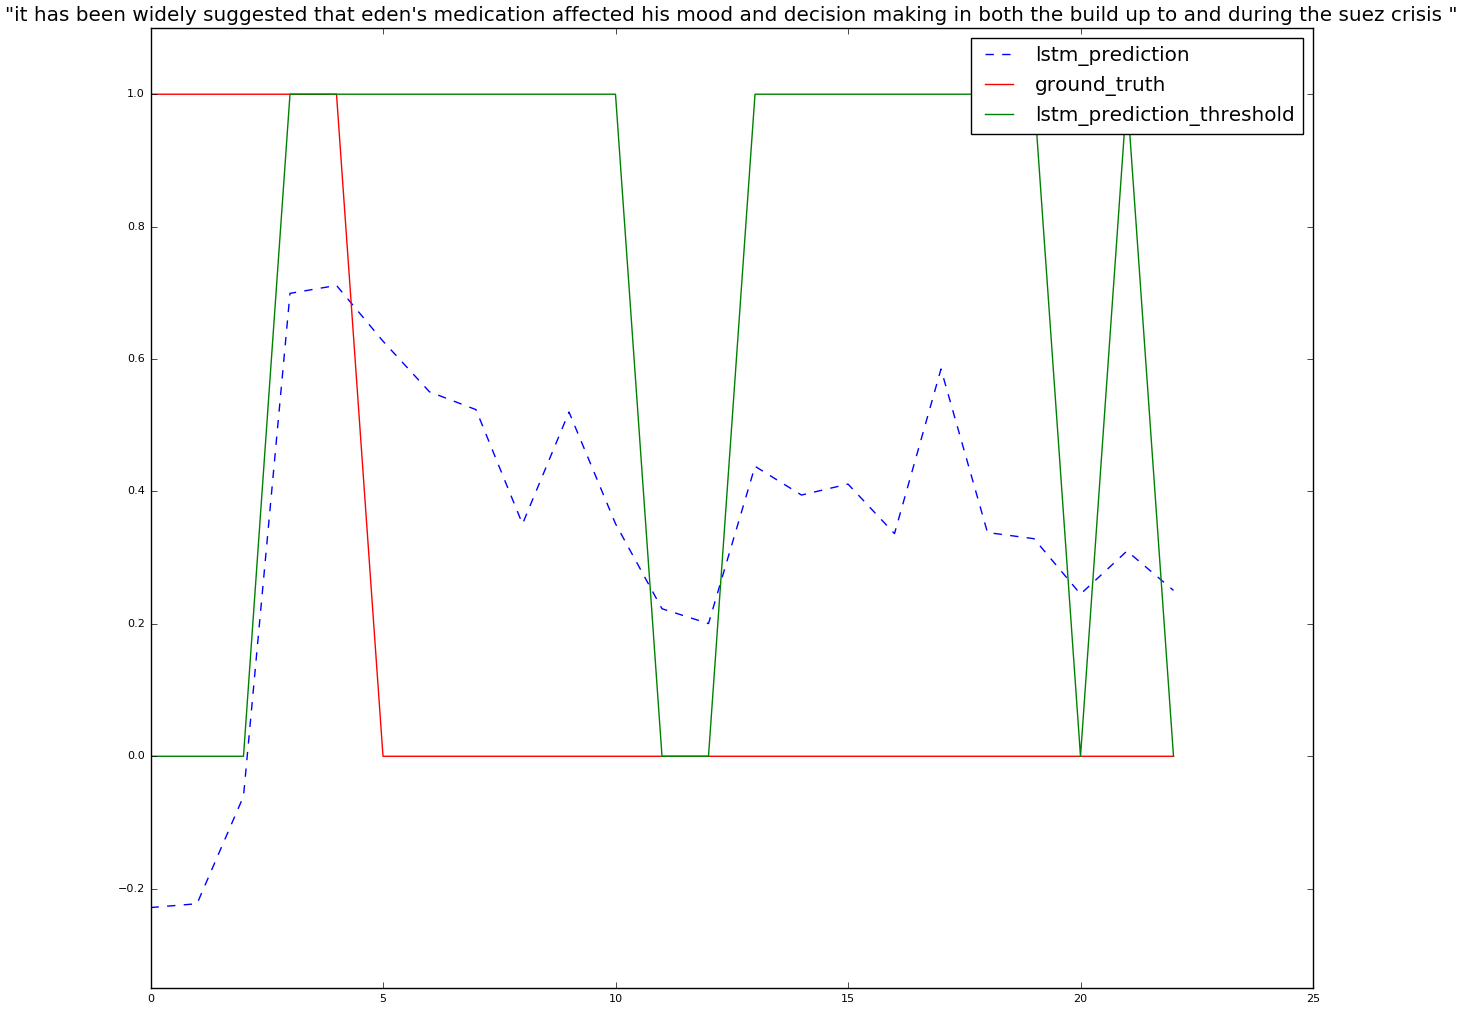
\includegraphics[scale=0.3]{images/task2_1dir/35_type1}
	\end{figure}
\end{frame}
\begin{frame}{Results for In-Sentence Cue Detection}
	\begin{figure}[htbp]
		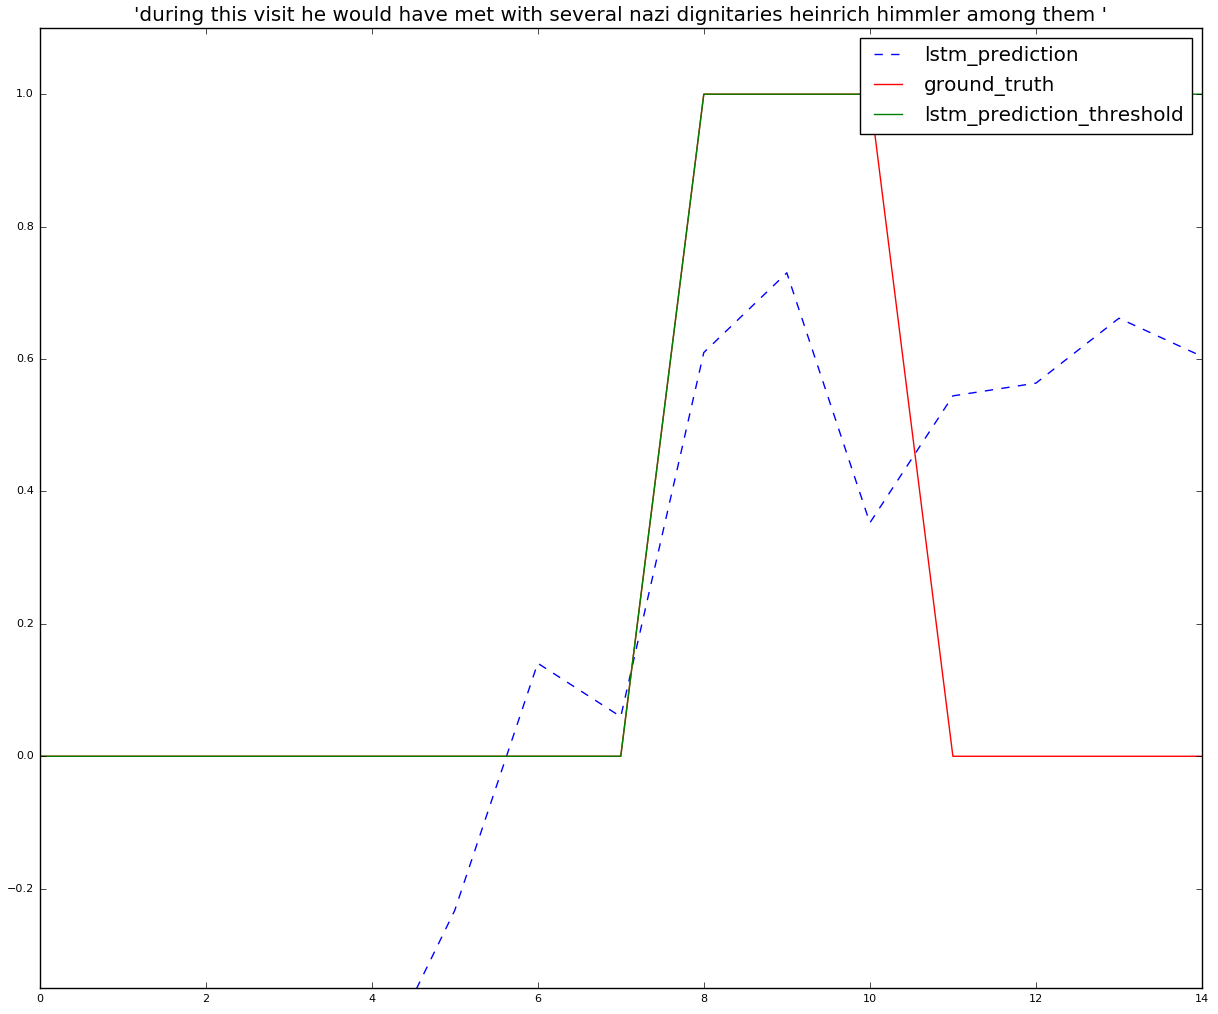
\includegraphics[scale=0.3]{images/task2_1dir/78_type1}
	\end{figure}
\end{frame}
\begin{frame}{Results for In-Sentence Cue Detection}
	\begin{figure}[htbp]
		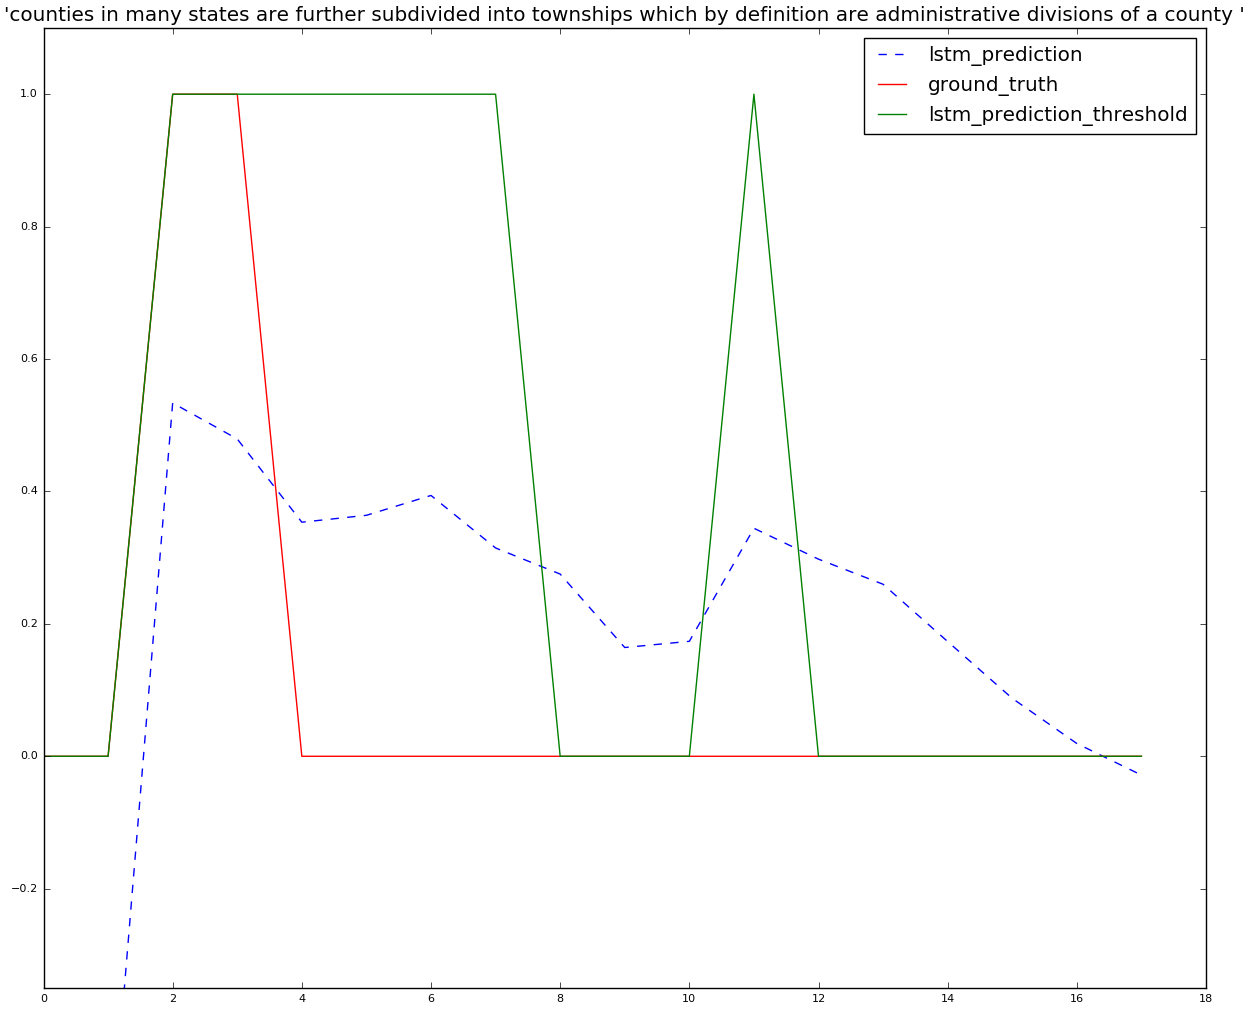
\includegraphics[scale=0.3]{images/task2_1dir/85_type1}
	\end{figure}
\end{frame}
\begin{frame}{Results for In-Sentence Cue Detection}
	\begin{figure}[htbp]
		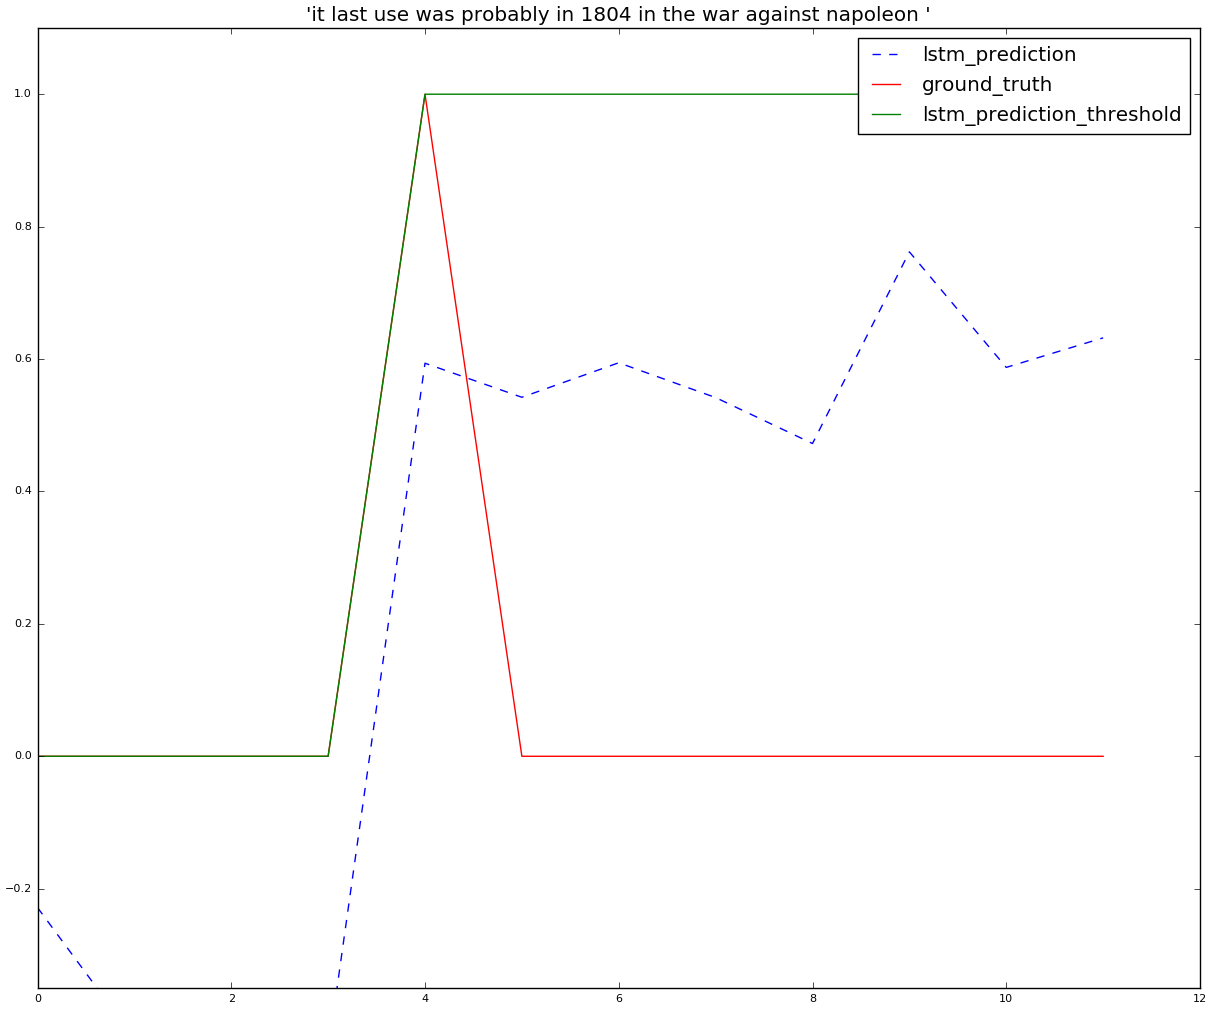
\includegraphics[scale=0.3]{images/task2_1dir/15_type1}
	\end{figure}
\end{frame}
%\begin{frame}{Results for In-Sentence Cue Detection}
%	In next slide we show some results with bidirectional model.
%\end{frame}
\begin{frame}{Results for In-Sentence Cue Detection (BLSTM)}
	\begin{figure}[htbp]
		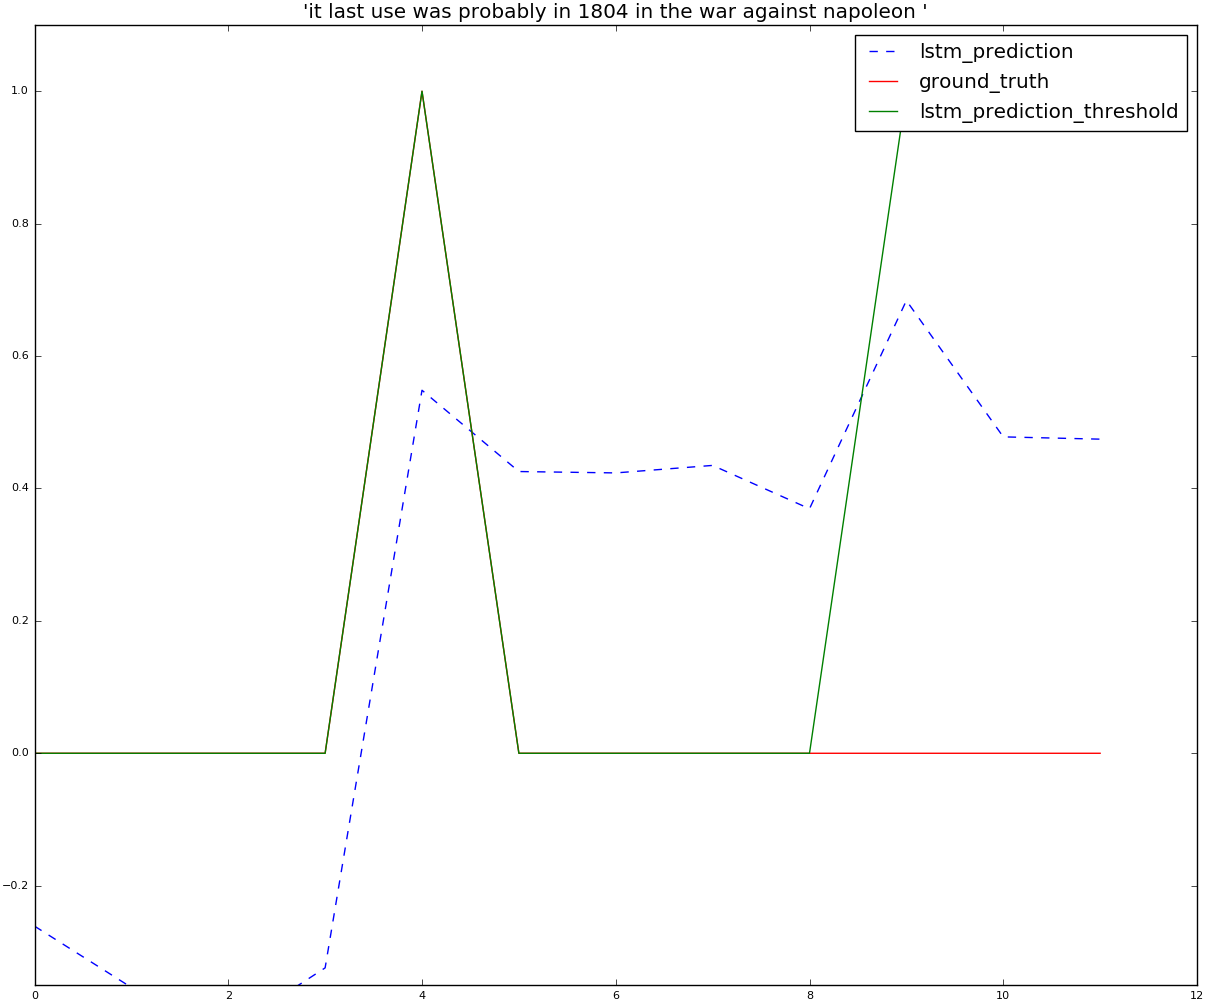
\includegraphics[scale=0.3]{images/task2_2dir/11_type1}
	\end{figure}
\end{frame}
\begin{frame}{Results for In-Sentence Cue Detection (BLSTM)}
	\begin{figure}[htbp]
		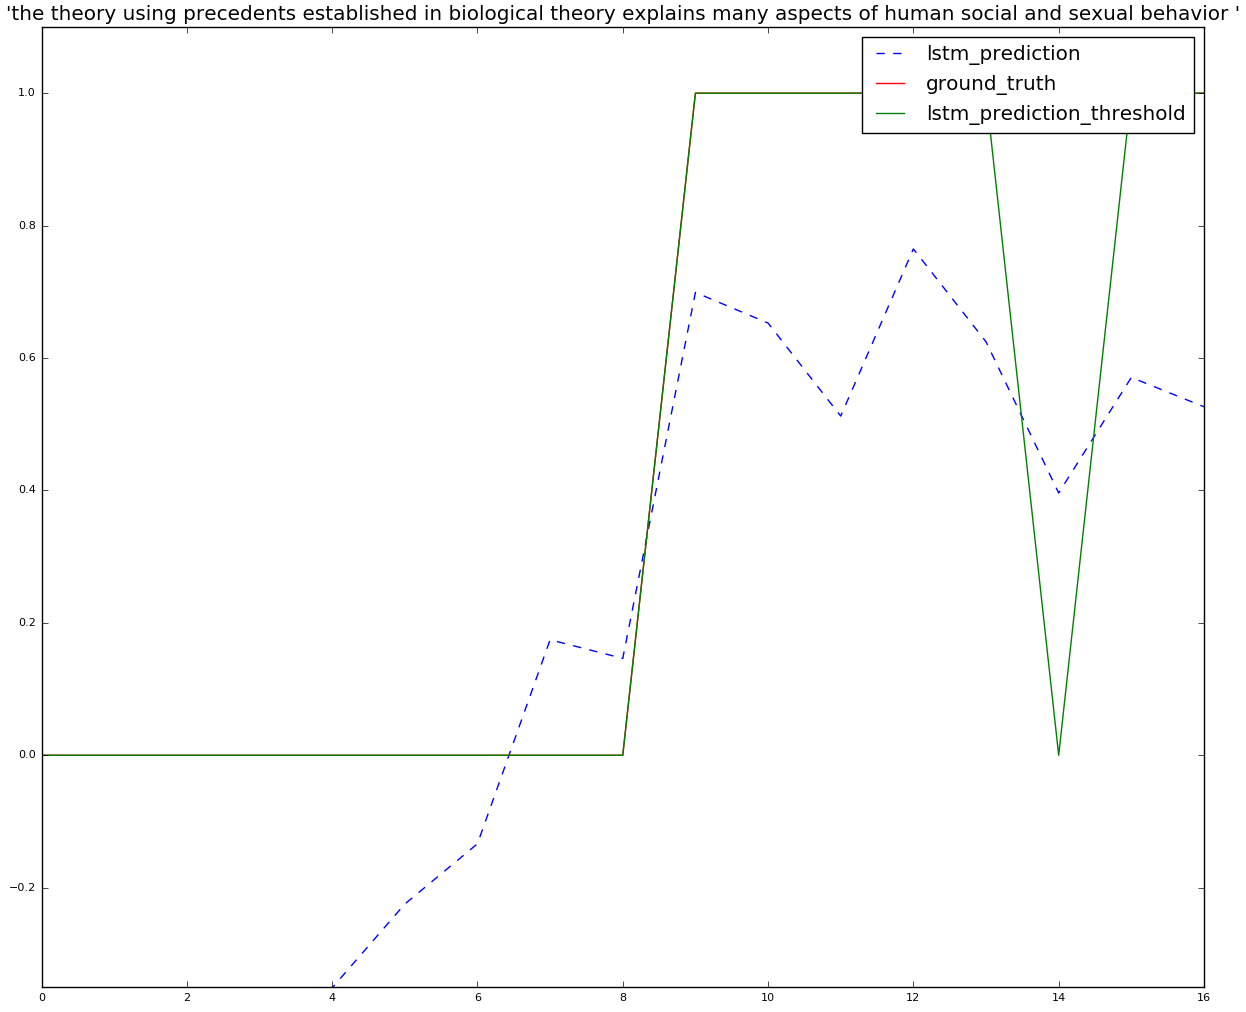
\includegraphics[scale=0.3]{images/task2_2dir/18_type1}
	\end{figure}
\end{frame}
\begin{frame}{Results for In-Sentence Cue Detection (BLSTM)}
	\begin{figure}[htbp]
		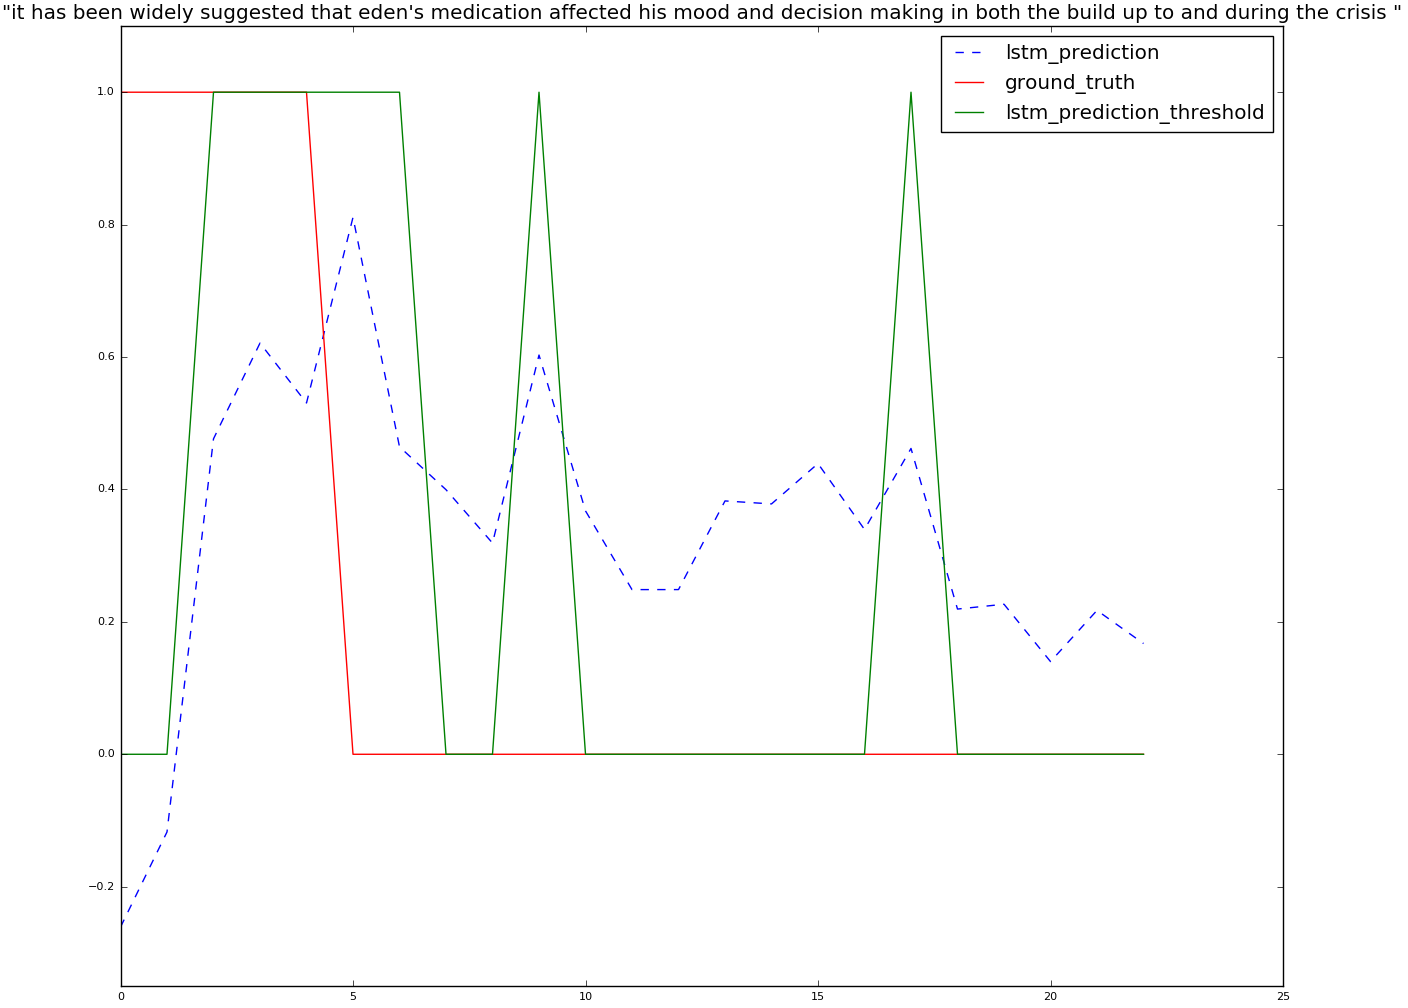
\includegraphics[scale=0.3]{images/task2_2dir/29_type1}
	\end{figure}
\end{frame}
\begin{frame}{Results for In-Sentence Cue Detection (BLSTM)}
	\begin{figure}[htbp]
		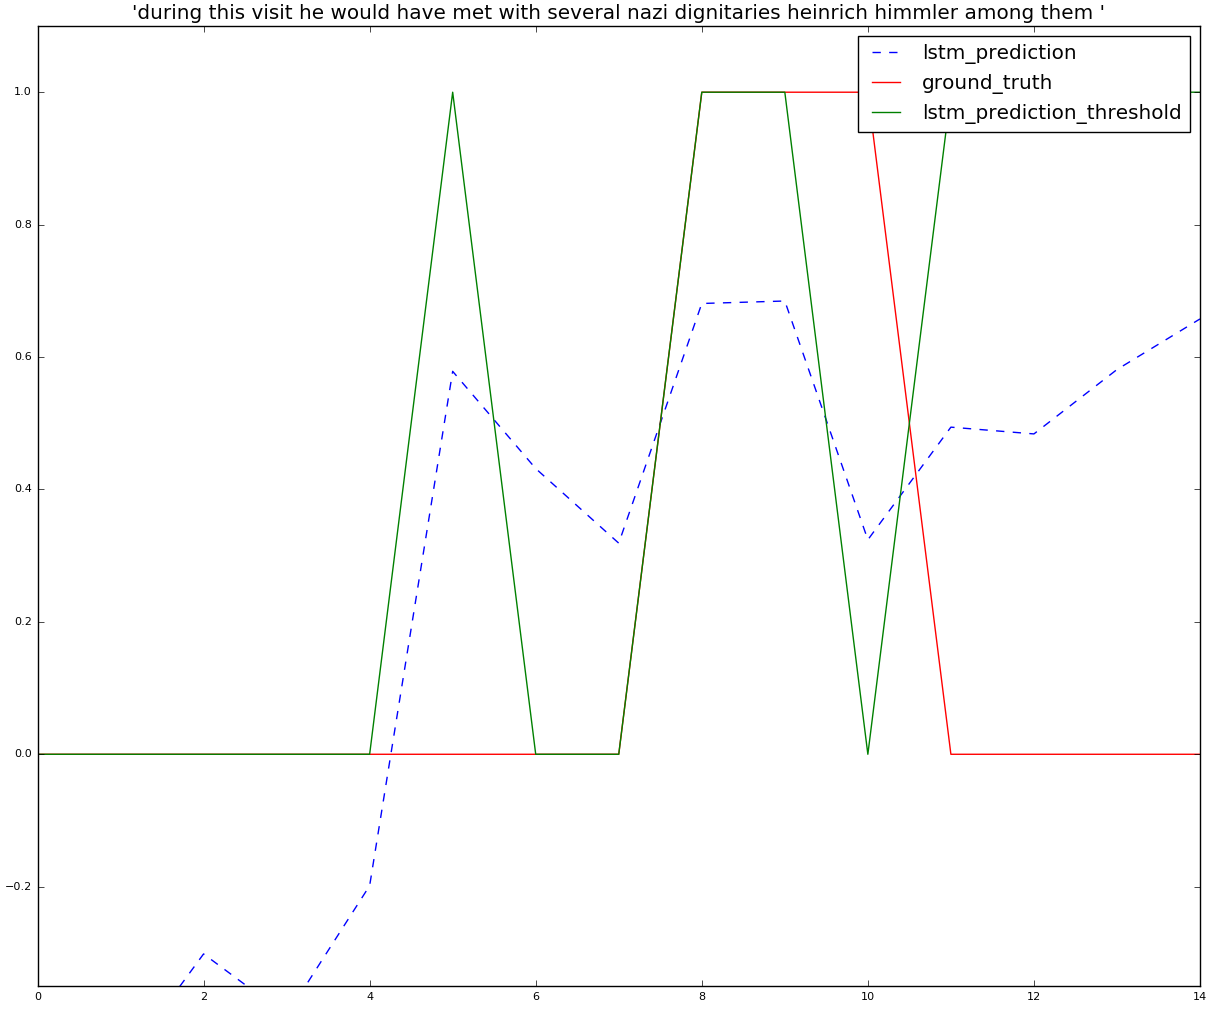
\includegraphics[scale=0.3]{images/task2_2dir/61_type1}
	\end{figure}
\end{frame}
\begin{frame}{Results for In-Sentence Cue Detection (BLSTM)}
	\begin{figure}[htbp]
		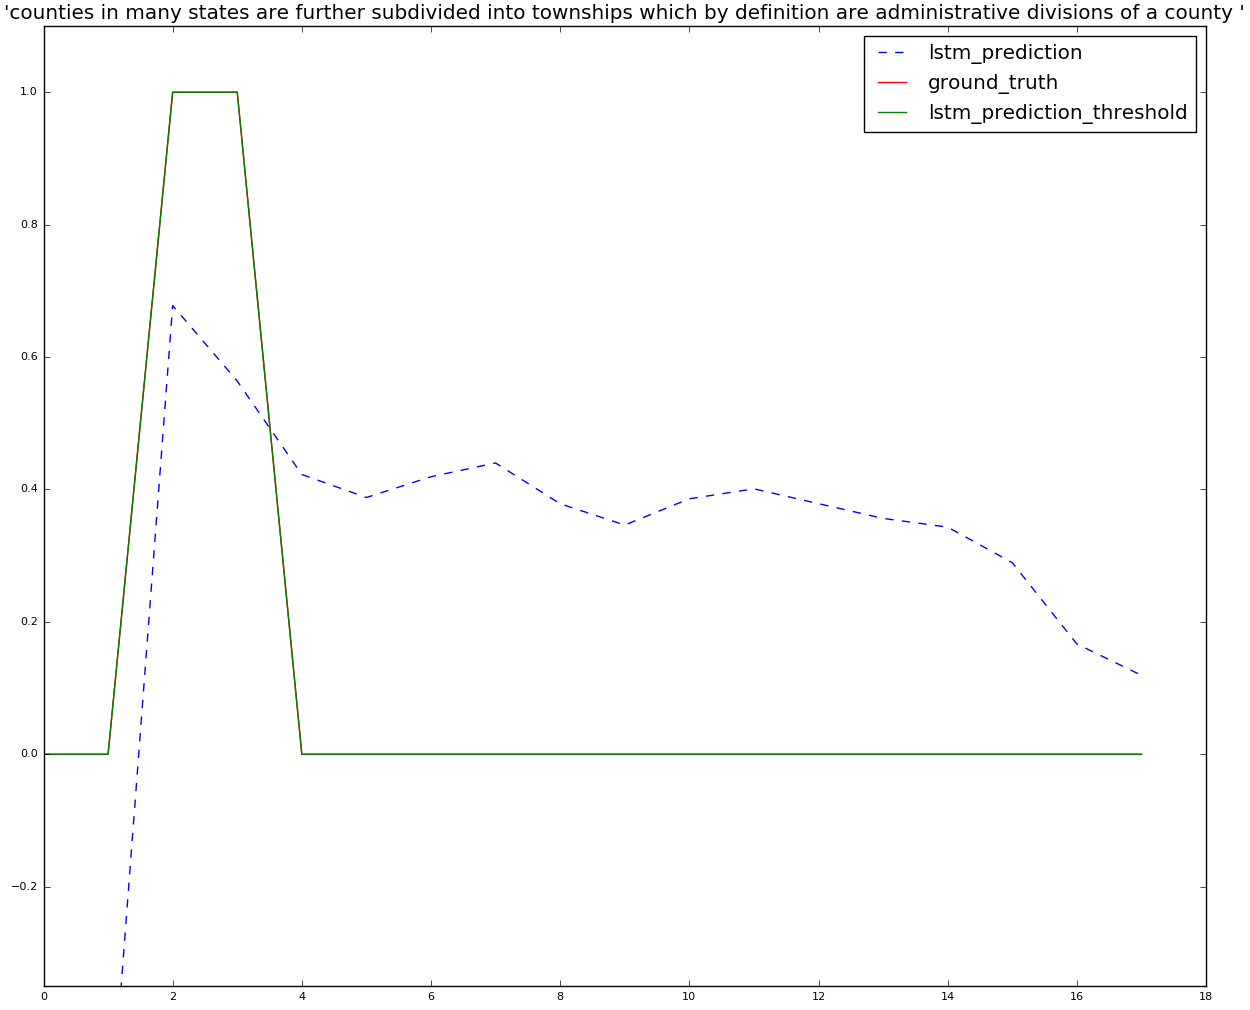
\includegraphics[scale=0.3]{images/task2_2dir/67_type1}
	\end{figure}
\end{frame}
\begin{frame}{Results for In-Sentence Cue Detection (BLSTM)}
	\begin{figure}[htbp]
		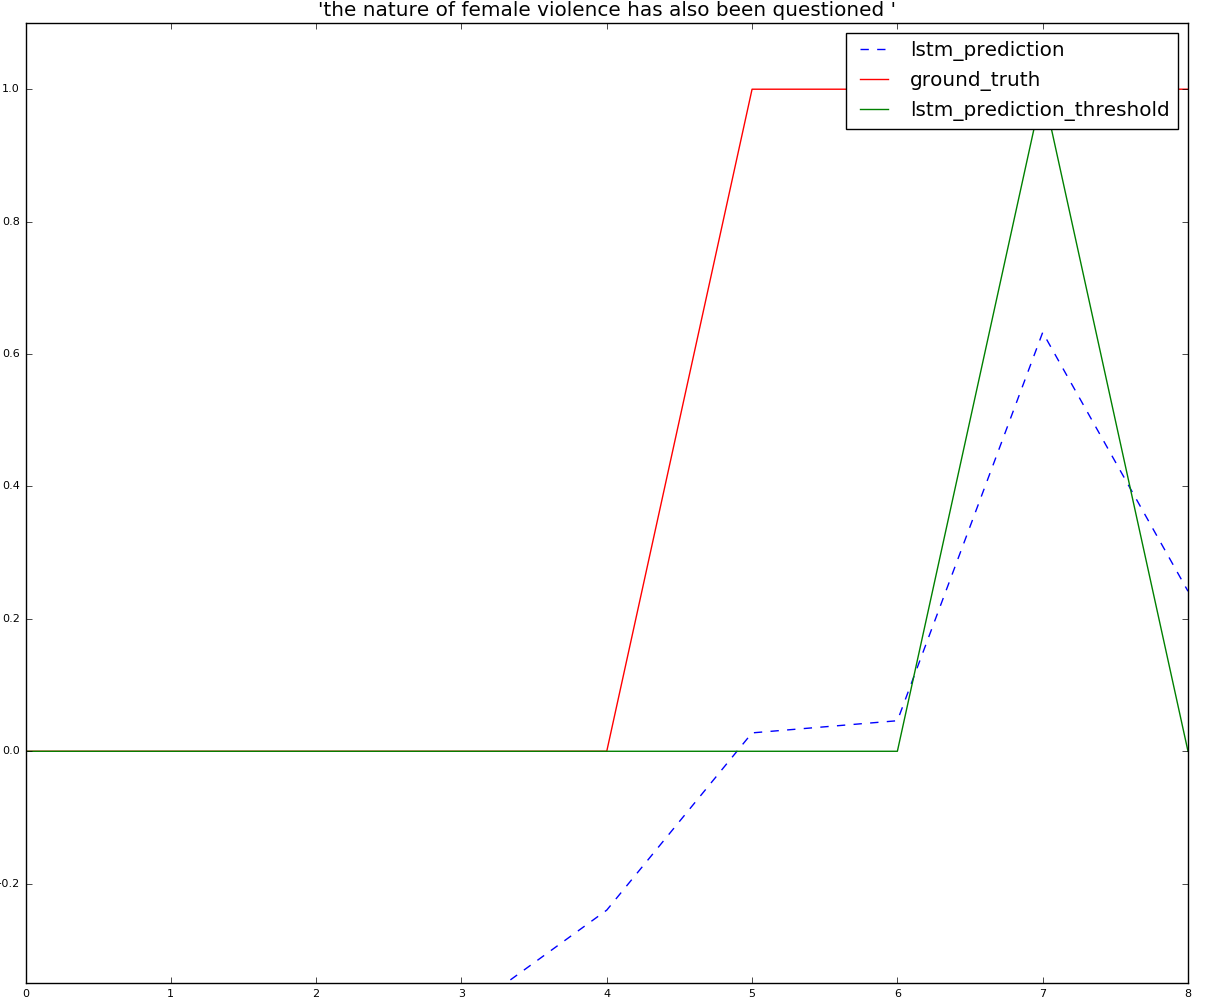
\includegraphics[scale=0.3]{images/task2_2dir/73_type1}
	\end{figure}
\end{frame}

\section{Conclusions}
\begin{frame}{Conclusions and Further Work}
	\begin{itemize}%setlength\itemsep{1em}
		\item In this project we have shown how RNNs, particularly LSTMs, can be used to classify sentences with satisfying results.	
		\item Moreover, embedding initial weights, learned by GloVe vectors, can mildly improve the learning speed and $F$-score of our model.
		\item Bidirectional model generally improve performances w.r.t. unidirectional, but the training is more slow.
		\item Contrary to intuition, the bidirectional model is able to capture information even looking the sentence in reverse. 
	\end{itemize}
	Future developments can be:
	\begin{itemize}
		\item Test the model on a different dataset.
		\item Optimize hyperparameters using a $k$-fold cross-validation on all cases.
		\item Variable threshold for in-sentence cue detection based on LSTM's output weights.
	\end{itemize}
\end{frame}

	
\end{document} 